% Select document class: uncomment one of the following
\documentclass[aspectratio=169]{beamer}  % For presentation mode
%\documentclass[11pt]{article}            % For article mode
%\usepackage{beamerarticle}               % Uncomment with article class

% =============================================================================
% COMMON PREAMBLE
% =============================================================================
% =============================================================================
% Common Preamble for Network+ Lecture Series
% This file provides consistent formatting, colors, packages, and styles
% across all lecture modules for both beamer presentations and article mode
% =============================================================================

% =============================================================================
% THEME AND COLORS
% =============================================================================
\usetheme{Madrid}
\usecolortheme{whale}

% Custom colors - standardized across all lectures
\definecolor{rctcblue}{RGB}{0, 74, 136}
\definecolor{rctcgold}{RGB}{255, 199, 44}
\definecolor{networkgreen}{RGB}{0, 128, 64}
\definecolor{alertred}{RGB}{180, 0, 0}
\definecolor{aborange}{RGB}{230, 126, 34}
\definecolor{copperbrown}{RGB}{184, 115, 51}
\definecolor{faborange}{RGB}{255, 165, 0}
\definecolor{fiberyellow}{RGB}{255, 215, 0}
\definecolor{shirepurple}{RGB}{102, 51, 153}
\definecolor{ipblue}{RGB}{52, 152, 219}
\definecolor{ippurple}{RGB}{155, 89, 182}
\definecolor{vlangreen}{RGB}{39, 174, 96}
\definecolor{tcpblue}{RGB}{30, 100, 180}
\definecolor{udpgreen}{RGB}{50, 160, 80}
\definecolor{dhcppurple}{RGB}{120, 60, 160}
\definecolor{dnsyellow}{RGB}{200, 170, 50}
\definecolor{batblack}{RGB}{30, 30, 40}
\definecolor{gothamgray}{RGB}{80, 85, 95}
\definecolor{paddysgreen}{RGB}{19, 77, 33}
\definecolor{beerlight}{RGB}{255, 199, 44}
\definecolor{sunnyorange}{RGB}{255, 140, 0}
\definecolor{ogregreen}{RGB}{34, 139, 34}
\definecolor{swampbrown}{RGB}{101, 67, 33}

% Set theme colors
\setbeamercolor{palette primary}{bg=rctcblue,fg=white}
\setbeamercolor{palette secondary}{bg=rctcblue!80,fg=white}
\setbeamercolor{palette tertiary}{bg=rctcblue!60,fg=white}
\setbeamercolor{structure}{fg=rctcblue}
\setbeamercolor{title}{fg=white,bg=rctcblue}
\setbeamercolor{frametitle}{fg=white,bg=rctcblue}
\setbeamercolor{block title}{bg=rctcblue,fg=white}
\setbeamercolor{block body}{bg=rctcblue!10,fg=black}
\setbeamercolor{block title alerted}{bg=alertred,fg=white}
\setbeamercolor{block body alerted}{bg=alertred!10,fg=black}
\setbeamercolor{block title example}{bg=networkgreen,fg=white}
\setbeamercolor{block body example}{bg=networkgreen!10,fg=black}

% =============================================================================
% PACKAGES
% =============================================================================
\usepackage[utf8]{inputenc}
\usepackage[T1]{fontenc}
\usepackage{lmodern}  % Better font rendering
\usepackage{graphicx}
\usepackage{tikz}
\usepackage{booktabs}
\usepackage{array}
\usepackage{multirow}
\usepackage{hyperref}
\usepackage{adjustbox}
\usepackage{amssymb}
\usepackage{amsmath}
\usepackage{calc}
\usepackage{fontawesome5}
% xcolor with [table] option: avoid colortbl.4ht hook conflict in tex4ht
\ifdefined\HCode
  \usepackage{xcolor}
  \usepackage{colortbl}  % provides \rowcolor etc.
\else
  \usepackage[table]{xcolor}  % includes colortbl for pdflatex
\fi

% =============================================================================
% TIKZ LIBRARIES AND SETUP
% =============================================================================
\usetikzlibrary{
    shapes.geometric,
    shapes.symbols,
    shapes.misc,
    arrows.meta,
    positioning,
    calc,
    fit,
    backgrounds,
    decorations.pathreplacing,
    decorations.pathmorphing,
    matrix,
    chains
}
% shadows library causes pgfuseshading errors with tex4ht;
% only load it when NOT building HTML
\ifdefined\HCode\else
    \usetikzlibrary{shadows}
\fi

% Graphics path for icons and chapter images
\graphicspath{
    {../images/icons/}
    {./images/icons/}
    {images/icons/}
    {../images/ch1/}
    {./images/ch1/}
    {images/ch1/}
    {../images/ch2/}
    {./images/ch2/}
    {images/ch2/}
    {../images/ch3/}
    {./images/ch3/}
    {images/ch3/}
    {../images/ch4/}
    {./images/ch4/}
    {images/ch4/}
    {../images/ch5/}
    {./images/ch5/}
    {images/ch5/}
    {../images/ch6/}
    {./images/ch6/}
    {images/ch6/}
    {../images/ch7/}
    {./images/ch7/}
    {images/ch7/}
    {../images/ch8/}
    {./images/ch8/}
    {images/ch8/}
    {../images/ch9/}
    {./images/ch9/}
    {images/ch9/}
    {../images/}
    {./images/}
    {images/}
}

% =============================================================================
% NETWORK DIAGRAM STYLES
% =============================================================================
\tikzset{
    % Node styles for network devices
    device/.style={
        inner sep=2pt,
        label distance=2pt
    },
    pc/.style={device},
    laptop/.style={device},
    server/.style={device},
    router/.style={device},
    switch/.style={device},
    firewall/.style={device},
    cloud/.style={device},
    phone/.style={device},
    tablet/.style={device},
    wifi/.style={device},
    % Connection styles
    ethernet/.style={
        draw=rctcblue,
        line width=1.5pt,
        -{Stealth[length=3mm]}
    },
    ethernet noarrow/.style={
        draw=rctcblue,
        line width=1.5pt
    },
    wireless/.style={
        draw=aborange,
        line width=1.5pt,
        dashed,
        -{Stealth[length=3mm]}
    },
    wireless noarrow/.style={
        draw=aborange,
        line width=1.5pt,
        dashed
    },
    wan/.style={
        draw=alertred,
        line width=2pt,
        -{Stealth[length=3mm]}
    },
    wan noarrow/.style={
        draw=alertred,
        line width=2pt
    },
    copper/.style={
        draw=copperbrown,
        line width=2pt,
        -{Stealth[length=3mm]}
    },
    copper noarrow/.style={
        draw=copperbrown,
        line width=2pt
    },
    fiber/.style={
        draw=fiberyellow,
        line width=2pt,
        -{Stealth[length=3mm]}
    },
    fiber noarrow/.style={
        draw=fiberyellow,
        line width=2pt
    },
    trunk/.style={
        draw=shirepurple,
        line width=2pt,
        -{Stealth[length=3mm]}
    },
    trunk noarrow/.style={
        draw=shirepurple,
        line width=2pt
    },
    % Packet/segment styles
    pktseg/.style={
        draw=rctcblue,
        fill=rctcblue!10,
        minimum height=0.5cm,
        font=\tiny,
        rounded corners=2pt
    },
    pktseg tcp/.style={
        draw=tcpblue,
        fill=tcpblue!15,
        minimum height=0.5cm,
        font=\tiny,
        rounded corners=2pt
    },
    pktseg udp/.style={
        draw=udpgreen,
        fill=udpgreen!15,
        minimum height=0.5cm,
        font=\tiny,
        rounded corners=2pt
    },
    pktseg highlight/.style={
        draw=aborange,
        fill=aborange!20,
        minimum height=0.5cm,
        font=\tiny,
        rounded corners=2pt
    },
    % Box styles
    ipbox/.style={
        draw=rctcblue,
        fill=rctcblue!10,
        rounded corners,
        minimum height=0.4cm,
        font=\small
    },
    portbox/.style={
        draw=tcpblue,
        fill=tcpblue!10,
        rounded corners,
        minimum height=0.4cm,
        font=\small
    },
    dnsbox/.style={
        draw=dnsyellow,
        fill=dnsyellow!15,
        rounded corners,
        minimum height=0.4cm,
        font=\small
    },
    routetable/.style={
        draw=rctcblue,
        fill=rctcblue!10,
        rounded corners,
        minimum height=0.4cm,
        font=\small
    },
    macbox/.style={
        draw=networkgreen,
        fill=networkgreen!10,
        rounded corners,
        minimum height=0.4cm,
        font=\small
    },
    % Frame segment styles (Ethernet frame diagrams)
    frameseg/.style={
        draw=rctcblue,
        fill=rctcblue!10,
        minimum height=0.5cm,
        font=\tiny,
        rounded corners=2pt
    },
    frameseg highlight/.style={
        draw=aborange,
        fill=aborange!20,
        minimum height=0.5cm,
        font=\tiny,
        rounded corners=2pt
    },
    % Process/flow styles
    process/.style={
        draw=rctcblue,
        fill=rctcblue!15,
        rounded corners,
        minimum width=2cm,
        minimum height=0.6cm,
        font=\small,
        align=center
    },
    decision/.style={
        draw=aborange,
        fill=aborange!15,
        diamond,
        aspect=2,
        minimum width=1.5cm,
        font=\small,
        align=center
    },
    % OSI Layer styles
    osilayer/.style={
        draw=rctcblue,
        fill=rctcblue!10,
        minimum width=3cm,
        minimum height=0.45cm,
        font=\small
    },
    osilayer highlight/.style={
        draw=aborange,
        fill=aborange!20,
        line width=1.5pt,
        minimum width=3cm,
        minimum height=0.45cm,
        font=\small\bfseries
    }
}

% =============================================================================
% ICON COMMANDS - Standardized using PNG files and FontAwesome
% =============================================================================
% Network device icons (PNG)
\newcommand{\iconpc}[1][0.6cm]{\resizebox{#1}{!}{
\includegraphics{icon_pc}}}
\newcommand{\iconlaptop}[1][0.6cm]{\resizebox{#1}{!}{
\includegraphics{icon_laptop}}}
\newcommand{\iconserver}[1][0.6cm]{\resizebox{#1}{!}{
\includegraphics{icon_server}}}
\newcommand{\iconrouter}[1][0.6cm]{\resizebox{#1}{!}{
\includegraphics{icon_router}}}
\newcommand{\iconswitch}[1][0.6cm]{\resizebox{#1}{!}{
\includegraphics{icon_switch}}}
\newcommand{\iconfirewall}[1][0.6cm]{\resizebox{#1}{!}{
\includegraphics{icon_firewall}}}
\newcommand{\iconcloud}[1][0.6cm]{\resizebox{#1}{!}{
\includegraphics{icon_cloud}}}
\newcommand{\iconphone}[1][0.6cm]{\resizebox{#1}{!}{
\includegraphics{icon_phone}}}
\newcommand{\icontablet}[1][0.6cm]{\resizebox{#1}{!}{
\includegraphics{icon_tablet}}}
\newcommand{\iconwifi}[1][0.6cm]{\resizebox{#1}{!}{
\includegraphics{icon_wifi}}}
\newcommand{\icondatabase}[1][0.6cm]{\resizebox{#1}{!}{
\includegraphics{icon_db}}}
\newcommand{\iconlock}[1][0.6cm]{\resizebox{#1}{!}{
\includegraphics{icon_lock}}}

% For HTML/tex4ht builds: replace PNG icons with FontAwesome5 glyphs.
% dvisvgm embeds font glyphs as vectors but silently ignores em:graph (PNG)
% specials, so PNG icons would be blank in the output SVGs. FA5 glyphs work.
\ifdefined\HCode
  \renewcommand{\iconpc}[1][0.6cm]{\resizebox{#1}{!}{\faIcon{desktop}}}
  \renewcommand{\iconlaptop}[1][0.6cm]{\resizebox{#1}{!}{\faIcon{laptop}}}
  \renewcommand{\iconserver}[1][0.6cm]{\resizebox{#1}{!}{\faIcon{server}}}
  \renewcommand{\iconrouter}[1][0.6cm]{\resizebox{#1}{!}{\faIcon{route}}}
  \renewcommand{\iconswitch}[1][0.6cm]{\resizebox{#1}{!}{\faIcon{network-wired}}}
  \renewcommand{\iconfirewall}[1][0.6cm]{\resizebox{#1}{!}{\faIcon{shield-alt}}}
  \renewcommand{\iconcloud}[1][0.6cm]{\resizebox{#1}{!}{\faIcon{cloud}}}
  \renewcommand{\iconphone}[1][0.6cm]{\resizebox{#1}{!}{\faIcon{mobile-alt}}}
  \renewcommand{\icontablet}[1][0.6cm]{\resizebox{#1}{!}{\faIcon{tablet-alt}}}
  \renewcommand{\iconwifi}[1][0.6cm]{\resizebox{#1}{!}{\faIcon{wifi}}}
  \renewcommand{\icondatabase}[1][0.6cm]{\resizebox{#1}{!}{\faIcon{database}}}
  \renewcommand{\iconlock}[1][0.6cm]{\resizebox{#1}{!}{\faIcon{lock}}}
\fi

% FontAwesome icons
\newcommand{\iconuser}[1][0.6cm]{\resizebox{#1}{!}{\faIcon{user}}}
\newcommand{\iconglobe}[1][0.6cm]{\resizebox{#1}{!}{\faIcon{globe}}}
\newcommand{\iconclock}[1][0.6cm]{\resizebox{#1}{!}{\faIcon{clock}}}
\newcommand{\iconmail}[1][0.6cm]{\resizebox{#1}{!}{\faIcon{envelope}}}
\newcommand{\icondoc}[1][0.6cm]{\resizebox{#1}{!}{\faIcon{file-alt}}}
\newcommand{\iconsearch}[1][0.6cm]{\resizebox{#1}{!}{\faIcon{search}}}
\newcommand{\icontools}[1][0.6cm]{\resizebox{#1}{!}{\faIcon{tools}}}
\newcommand{\iconchart}[1][0.6cm]{\resizebox{#1}{!}{\faIcon{chart-line}}}
\newcommand{\iconalert}[1][0.6cm]{\resizebox{#1}{!}{\faIcon{bell}}}
\newcommand{\iconlog}[1][0.6cm]{\resizebox{#1}{!}{\faIcon{clipboard-list}}}
\newcommand{\iconeye}[1][0.6cm]{\resizebox{#1}{!}{\faIcon{eye}}}
\newcommand{\iconhacker}[1][0.6cm]{\resizebox{#1}{!}{\faIcon{user-secret}}}
\newcommand{\iconkey}[1][0.6cm]{\resizebox{#1}{!}{\faIcon{key}}}
\newcommand{\iconfile}[1][0.6cm]{\resizebox{#1}{!}{\faIcon{file-alt}}}
\newcommand{\icondog}[1][0.6cm]{\resizebox{#1}{!}{\faIcon{dog}}}
\newcommand{\iconcat}[1][0.6cm]{\resizebox{#1}{!}{\faIcon{cat}}}
\newcommand{\iconvoip}[1][0.6cm]{\resizebox{#1}{!}{\faIcon{phone-volume}}}
\newcommand{\iconmoney}[1][0.6cm]{\resizebox{#1}{!}{\faIcon{money-bill-wave}}}
\newcommand{\icontrash}[1][0.6cm]{\resizebox{#1}{!}{\faIcon{trash}}}
\newcommand{\iconbuilding}[1][0.6cm]{\resizebox{#1}{!}{\faIcon{building}}}

% =============================================================================
% CUSTOM COMMANDS AND ENVIRONMENTS
% =============================================================================

% Key term formatting
\newcommand{\keyterm}[1]{\textbf{#1}}

% Slide section marker
\newcommand{\sectionslide}[1]{
    \begin{frame}
        \vfill
        \centering
        \begin{beamercolorbox}[sep=8pt,center,shadow=true,rounded=true]{title}
            \usebeamerfont{title}\Huge #1
        \end{beamercolorbox}
        \vfill
    \end{frame}
}

% Case study frame environment
\newenvironment{casestudy}[1]{%
    \begin{alertblock}{$\blacktriangleright$ Case Study: #1}
}{%
    \end{alertblock}
}

% Solution frame environment  
\newenvironment{casesolution}[1]{%
    \begin{exampleblock}{$\checkmark$ Solution: #1}
}{%
    \end{exampleblock}
}

% =============================================================================
% FOOTER WITH SLIDE NUMBERS
% =============================================================================
\setbeamertemplate{footline}{
    \leavevmode%
    \hbox{%
        \begin{beamercolorbox}[wd=.333333\paperwidth,ht=2.25ex,dp=1ex,center]{author in head/foot}%
            \usebeamerfont{author in head/foot}\insertshortauthor
        \end{beamercolorbox}%
        \begin{beamercolorbox}[wd=.333333\paperwidth,ht=2.25ex,dp=1ex,center]{title in head/foot}%
            \usebeamerfont{title in head/foot}\insertshorttitle
        \end{beamercolorbox}%
        \begin{beamercolorbox}[wd=.333333\paperwidth,ht=2.25ex,dp=1ex,right]{date in head/foot}%
            \usebeamerfont{date in head/foot}\insertshortdate{}\hspace*{2em}
            \insertframenumber{} / \inserttotalframenumber\hspace*{2ex}
        \end{beamercolorbox}}%
    \vskip0pt%
}

% =============================================================================
% ARTICLE MODE SUPPORT
% =============================================================================
% The following commands help with beamerarticle mode for HTML conversion

% In article mode, add proper section/subsection support and override environments
\mode<article>{
    % Make sure figure captions work properly
    \setbeamertemplate{caption}[numbered]
    \setbeamertemplate{caption label separator}{: }
    
    % Add some spacing for readability
    \setlength{\parskip}{0.5em}
    \setlength{\parindent}{0pt}
    
    % Article mode versions of case study environments
    \renewenvironment{casestudy}[1]{%
        \vspace{0.3cm}\noindent\textbf{Case Study: #1}\newline\begin{itshape}
    }{%
        \end{itshape}\vspace{0.3cm}
    }
    
    \renewenvironment{casesolution}[1]{%
        \vspace{0.3cm}\noindent\textbf{Solution: #1}\newline\begin{itshape}
    }{%
        \end{itshape}\vspace{0.3cm}
    }
}

% Command to mark content that only appears in article mode
\newcommand{\articleonly}[1]{\mode<article>{#1}}

% Command to mark content that only appears in presentation mode
\newcommand{\presentationonly}[1]{\mode<presentation>{#1}}


% =============================================================================
% DOCUMENT INFO
% =============================================================================
\title[Network+ Module 5.0]{Routing, Switching, and Network Infrastructure}
\subtitle{Intro to Networks Module 5.0}
\author[B. Shea]{Brendan Shea, PhD}
\institute[RCTC]{Rochester Community and Technical College\\Intro to Networking}
\date{}

% Article mode: figures will have specific contextual descriptions added inline

\begin{document}

% =============================================================================
% SLIDE 1: Title Slide
% =============================================================================
\begin{frame}
    \titlepage
    \begin{center}
        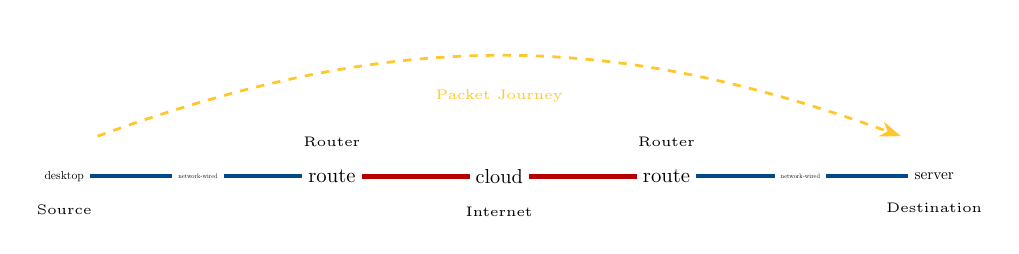
\begin{tikzpicture}[scale=0.85]
            % Source PC
            \node[pc] (pc1) at (0,0) {\iconpc[0.5cm]};
            \node[font=\tiny, below=0.1cm of pc1] {Source};
            
            % Switch 1
            \node[switch] (sw1) at (2,0) {\iconswitch[0.5cm]};
            
            % Router 1
            \node[router] (rtr1) at (4,0) {\iconrouter[0.6cm]};
            \node[font=\tiny, above=0.1cm of rtr1] {Router};
            
            % Cloud/Internet
            \node[cloud] (cloud) at (6.5,0) {\iconcloud[0.6cm]};
            \node[font=\tiny, below=0.1cm of cloud] {Internet};
            
            % Router 2
            \node[router] (rtr2) at (9,0) {\iconrouter[0.6cm]};
            \node[font=\tiny, above=0.1cm of rtr2] {Router};
            
            % Switch 2
            \node[switch] (sw2) at (11,0) {\iconswitch[0.5cm]};
            
            % Destination Server
            \node[server] (srv) at (13,0) {\iconserver[0.5cm]};
            \node[font=\tiny, below=0.1cm of srv] {Destination};
            
            % Connections
            \draw[ethernet noarrow] (pc1) -- (sw1);
            \draw[ethernet noarrow] (sw1) -- (rtr1);
            \draw[wan noarrow] (rtr1) -- (cloud);
            \draw[wan noarrow] (cloud) -- (rtr2);
            \draw[ethernet noarrow] (rtr2) -- (sw2);
            \draw[ethernet noarrow] (sw2) -- (srv);
            
            % Path arrow
            \draw[-{Stealth}, line width=1pt, rctcgold, dashed] 
                (0.5,0.6) to[bend left=20] (12.5,0.6);
            \node[font=\tiny, rctcgold] at (6.5,1.2) {Packet Journey};
        \end{tikzpicture}
    \end{center}

\articleonly{
\par\small\emph{This diagram illustrates a packet's journey through network infrastructure: source PC through Switch 1 to Router 1, across internet cloud to Router 2, through Switch 2 to destination server. The dashed golden arrow traces this path, showing how routing decisions forward traffic across network boundaries while Ethernet addresses change at each hop and IP addresses remain constant end-to-end.}\par
}

\end{frame}

% Table of contents in presentation mode only
\presentationonly{
\begin{frame}[allowframebreaks]{Outline}
\small
\tableofcontents[hideallsubsections]
\end{frame}
}


% =============================================================================
% SLIDE 2: Review - From IP Addressing to Routing
% =============================================================================
\section*{Review from Module 4}

\begin{frame}{Review: From IP Addressing to Routing}
    \begin{columns}[T]
        \begin{column}{0.55\textwidth}
            \begin{itemize}
                \item Module 4 covered \textbf{IP addresses} and \textbf{subnetting} (Layer 3 addressing).
                \item Today's question: How does data actually \textit{get} to its destination?
                \item IP addresses tell us \textbf{where} to go, but \keyterm{routing} tells us \textbf{how} to get there.
                \item Routers make decisions about the best path for each packet.
            \end{itemize}
            
            \vspace{0.3em}
            \begin{alertblock}{The Journey Ahead}
                \textbf{Module 4}: Addressing (naming the destination) \\
                \textbf{Module 5}: Routing (finding the path there)
            \end{alertblock}
        \end{column}
        \begin{column}{0.42\textwidth}
            \begin{center}
                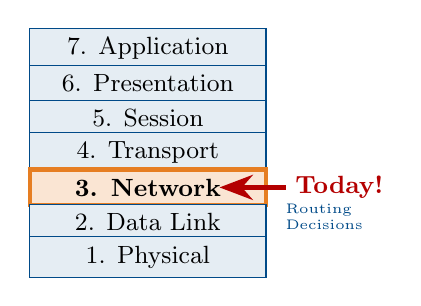
\begin{tikzpicture}[scale=0.7]
                    % OSI Stack
                    \node[osilayer] (l7) at (0, 3.15) {7. Application};
                    \node[osilayer] (l6) at (0, 2.52) {6. Presentation};
                    \node[osilayer] (l5) at (0, 1.89) {5. Session};
                    \node[osilayer] (l4) at (0, 1.26) {4. Transport};
                    \node[osilayer highlight] (l3) at (0, 0.63) {3. Network};
                    \node[osilayer] (l2) at (0, 0) {2. Data Link};
                    \node[osilayer] (l1) at (0, -0.63) {1. Physical};
                    
                    % Today's focus arrow
                    \draw[-{Stealth}, line width=2pt, alertred] (2.5, 0.63) -- (1.3, 0.63);
                    \node[right, font=\small\bfseries, alertred] at (2.5, 0.63) {Today!};
                    
                    % What we're covering
                    \node[font=\tiny, align=left, rctcblue] at (3.2, 0.1) {Routing\\Decisions};
                \end{tikzpicture}
            \end{center}
        \end{column}
    \end{columns}
\end{frame}

% =============================================================================
% SLIDE 3: Module Overview and Learning Outcomes
% =============================================================================
\begin{frame}[t,shrink=10]{Module Overview and Learning Outcomes}
    \begin{columns}[T]
        \begin{column}{0.48\textwidth}
            \begin{block}{Topics Covered}
                \begin{enumerate}
                    \item Routing Technologies and Tables
                    \item Dynamic Routing Protocols
                    \item Network Address Translation (NAT)
                    \item Firewalls and Security
                    \item Enterprise Network Topologies
                    \item Virtual LANs (VLANs)
                \end{enumerate}
            \end{block}
        \end{column}
        \begin{column}{0.48\textwidth}
            \begin{block}{Learning Outcomes}
                After this module, you will be able to:
                \begin{itemize}
                    \item Explain how routers forward packets using routing tables
                    \item Compare static vs.\ dynamic routing protocols
                    \item Describe NAT and PAT operation
                    \item Identify firewall types and proper placement
                    \item Design networks using three-tier hierarchy
                    \item Configure and troubleshoot VLANs
                \end{itemize}
            \end{block}
        \end{column}
    \end{columns}
\end{frame}



% =============================================================================
% SLIDE 5: The Router - Gateway Between Networks
% =============================================================================
\section{Routing Foundations}
\subsection{Routers and Path Selection}

\articleonly{
This section introduces router roles, routing tables, and packet forwarding behavior across network boundaries.
}

\begin{frame}{The Router: Gateway Between Networks}
    \begin{columns}[T]
        \begin{column}{0.48\textwidth}
            \begin{itemize}
                \item \keyterm{Routers} connect different networks at Layer 3.
                \item Each router interface has its own IP address on a \textbf{different subnet}.
                \item Routers make \keyterm{forwarding decisions} based on the destination IP address.
                \item Every packet passing through decrements its \textbf{TTL} by 1.
            \end{itemize}
            
            \vspace{0.3em}
            \begin{alertblock}{Key Difference from Switches}
                \small
                \textbf{Switches}: MAC addresses (Layer 2) \\
                \textbf{Routers}: IP addresses (Layer 3)
            \end{alertblock}
        \end{column}
        \begin{column}{0.48\textwidth}
            \begin{center}
                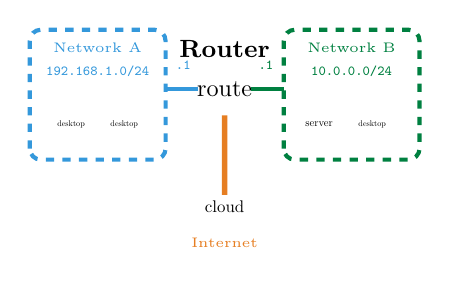
\begin{tikzpicture}[scale=0.75]
                    % Router in center
                    \node[router] (rtr) at (3,1.2) {\iconrouter[0.7cm]};
                    \node[font=\small\bfseries, above=0.1cm of rtr] {Router};
                    
                    % Network A (left)
                    \draw[dashed, ipblue, line width=1.5pt, rounded corners] 
                        (-0.3,0) rectangle (2,2.2);
                    \node[font=\tiny, ipblue] at (0.85,1.9) {Network A};
                    \node[font=\tiny\ttfamily, ipblue] at (0.85,1.5) {192.168.1.0/24};
                    
                    \node[pc] (pc1) at (0.4,0.6) {\iconpc[0.35cm]};
                    \node[pc] (pc2) at (1.3,0.6) {\iconpc[0.35cm]};
                    
                    % Network B (right)
                    \draw[dashed, networkgreen, line width=1.5pt, rounded corners] 
                        (4,0) rectangle (6.3,2.2);
                    \node[font=\tiny, networkgreen] at (5.15,1.9) {Network B};
                    \node[font=\tiny\ttfamily, networkgreen] at (5.15,1.5) {10.0.0.0/24};
                    
                    \node[server] (srv1) at (4.6,0.6) {\iconserver[0.35cm]};
                    \node[pc] (pc3) at (5.5,0.6) {\iconpc[0.35cm]};
                    
                    % Connections to router
                    \draw[ethernet noarrow, ipblue] (2,1.2) -- (2.55,1.2);
                    \draw[ethernet noarrow, networkgreen] (3.45,1.2) -- (4,1.2);
                    
                    % Interface labels
                    \node[font=\tiny\ttfamily, ipblue] at (2.3,1.6) {.1};
                    \node[font=\tiny\ttfamily, networkgreen] at (3.7,1.6) {.1};
                    
                    % Internet connection (below)
                    \node[cloud] (cloud) at (3,-0.8) {\iconcloud[0.5cm]};
                    \node[font=\tiny, aborange] at (3,-1.4) {Internet};
                    \draw[wan noarrow, aborange] (3,0.75) -- (cloud);
                \end{tikzpicture}
            \end{center}

\articleonly{
\par\small\emph{This diagram shows a router managing three connected interfaces: left interface connects to local LAN with PCs, right interface connects to server network, and WAN connection links to internet. Each interface has its own IP address and network identifier, allowing the router to switch traffic between networks and enabling inter-network communication.}\par
}

        \end{column}
    \end{columns}
\end{frame}

% =============================================================================
% SLIDE 6: Routing Tables and Path Selection
% =============================================================================
\begin{frame}{Routing Tables and Path Selection}
    \begin{columns}[T]
        \begin{column}{0.48\textwidth}
            \begin{itemize}
                \item Every router maintains a \keyterm{routing table} listing known networks.
                \item Key components of each entry:
                    \begin{itemize}
                        \item \textbf{Destination network} and prefix/mask
                        \item \textbf{Next hop} (next router's IP) OR exit interface
                        \item \textbf{Metric} (cost to reach destination)
                    \end{itemize}
                \item Router uses \keyterm{longest prefix match} to find best route.
            \end{itemize}
            
            \vspace{0.3em}
            \begin{exampleblock}{Longest Prefix Match}
                If a packet for \texttt{192.168.1.50} matches both \texttt{192.168.0.0/16} and \texttt{192.168.1.0/24}, the \textbf{/24 wins} because it's more specific.
            \end{exampleblock}
        \end{column}
        \begin{column}{0.48\textwidth}
            \begin{center}
                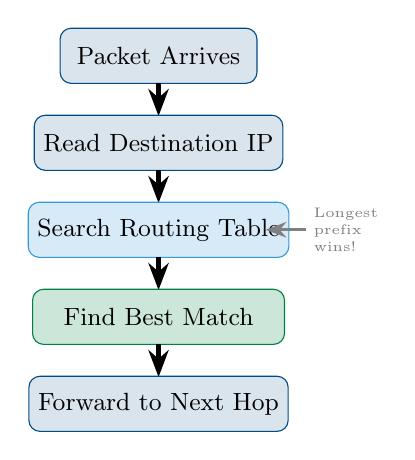
\begin{tikzpicture}[scale=0.85]
                    % Flowchart for routing decision
                    \node[draw=rctcblue, fill=rctcblue!15, rounded corners, 
                          minimum width=2.5cm, minimum height=0.7cm, font=\small] 
                          (step1) at (0,3.5) {Packet Arrives};
                    
                    \draw[-{Stealth}, line width=1.5pt] (0,3.1) -- (0,2.6);
                    
                    \node[draw=rctcblue, fill=rctcblue!15, rounded corners, 
                          minimum width=3cm, minimum height=0.7cm, font=\small, align=center] 
                          (step2) at (0,2.2) {Read Destination IP};
                    
                    \draw[-{Stealth}, line width=1.5pt] (0,1.8) -- (0,1.3);
                    
                    \node[draw=ipblue, fill=ipblue!20, rounded corners, 
                          minimum width=3cm, minimum height=0.7cm, font=\small, align=center] 
                          (step3) at (0,0.9) {Search Routing Table};
                    
                    \draw[-{Stealth}, line width=1.5pt] (0,0.5) -- (0,0);
                    
                    \node[draw=networkgreen, fill=networkgreen!20, rounded corners, 
                          minimum width=3.2cm, minimum height=0.7cm, font=\small, align=center] 
                          (step4) at (0,-0.4) {Find Best Match};
                    
                    \draw[-{Stealth}, line width=1.5pt] (0,-0.8) -- (0,-1.3);
                    
                    \node[draw=rctcblue, fill=rctcblue!15, rounded corners, 
                          minimum width=3.2cm, minimum height=0.7cm, font=\small, align=center] 
                          (step5) at (0,-1.7) {Forward to Next Hop};
                    
                    % Annotation
                    \node[font=\tiny, align=left, gray] at (2.8,0.9) {Longest\\prefix\\wins!};
                    \draw[-{Stealth}, gray, line width=1pt] (2.2,0.9) -- (1.6,0.9);
                \end{tikzpicture}
            \end{center}
        \end{column}
    \end{columns}
\end{frame}

% =============================================================================
% SLIDE 7: Static and Default Routes
% =============================================================================
\begin{frame}{Static and Default Routes}
    \begin{columns}[T]
        \begin{column}{0.48\textwidth}
            \begin{block}{Static Routes}
                \small
                \begin{itemize}\setlength{\itemsep}{2pt}
                    \item \textbf{Manually configured} by administrator
                    \item Don't change unless admin modifies
                    \item Good for: small networks, specific paths
                    \item Downside: won't adapt to failures
                \end{itemize}
                
                \vspace{0.2em}
                \ttfamily\footnotesize
                ip route 10.0.0.0 255.0.0.0 192.168.1.1
            \end{block}
            
            \vspace{0.2em}
            \begin{alertblock}{When to Use Static}
                \small
                Small networks, stub networks (one exit), or when you need security control over paths.
            \end{alertblock}
        \end{column}
        \begin{column}{0.48\textwidth}
            \begin{block}{Default Route}
                \small
                \begin{itemize}\setlength{\itemsep}{2pt}
                    \item The ``\keyterm{route of last resort}''
                    \item Used when \textbf{no specific match} found
                    \item Points to gateway for ``everything else''
                    \item Written as \texttt{0.0.0.0/0}
                \end{itemize}
                
                \vspace{0.2em}
                \ttfamily\footnotesize
                ip route 0.0.0.0 0.0.0.0 203.0.113.1
            \end{block}
            
            \vspace{0.2em}
            \begin{exampleblock}{Analogy}
                \small
                \textbf{Static}: ``Take Highway 10 to Grandma's.'' \\
                \textbf{Default}: ``For anywhere else, head to the main highway.''
            \end{exampleblock}
        \end{column}
    \end{columns}
\end{frame}

% =============================================================================
% SLIDE 8: Routing Table Example (DIAGRAM SLIDE)
% =============================================================================
\begin{frame}{Routing Table Example}
    \begin{center}
        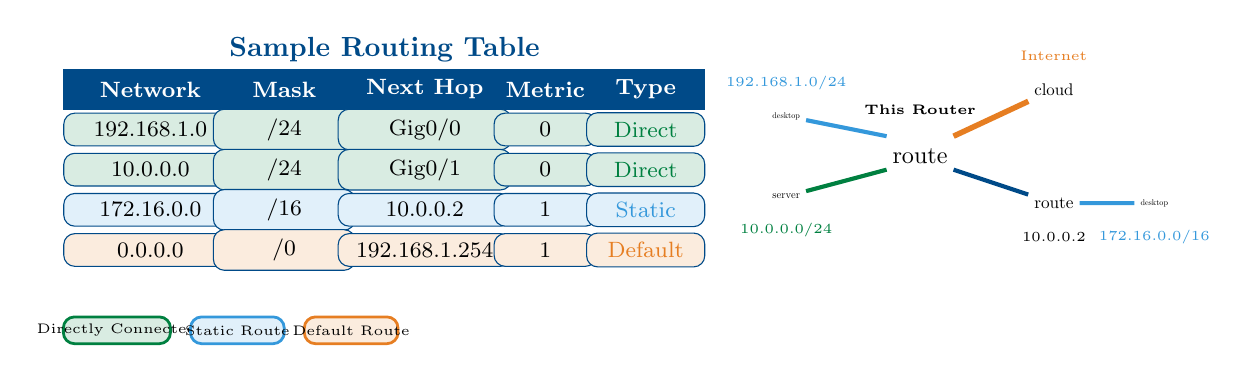
\begin{tikzpicture}[scale=0.85]
            % Routing table
            \node[font=\normalsize\bfseries, rctcblue] at (0,3.8) {Sample Routing Table};
            
            % Table header
            \node[draw=rctcblue, fill=rctcblue, minimum width=2.2cm, minimum height=0.5cm, 
                  font=\footnotesize\bfseries, text=white] (h1) at (-3.5,3.2) {Network};
            \node[draw=rctcblue, fill=rctcblue, minimum width=1.8cm, minimum height=0.5cm, 
                  font=\footnotesize\bfseries, text=white] (h2) at (-1.5,3.2) {Mask};
            \node[draw=rctcblue, fill=rctcblue, minimum width=2.2cm, minimum height=0.5cm, 
                  font=\footnotesize\bfseries, text=white] (h3) at (0.6,3.2) {Next Hop};
            \node[draw=rctcblue, fill=rctcblue, minimum width=1.3cm, minimum height=0.5cm, 
                  font=\footnotesize\bfseries, text=white] (h4) at (2.4,3.2) {Metric};
            \node[draw=rctcblue, fill=rctcblue, minimum width=1.5cm, minimum height=0.5cm, 
                  font=\footnotesize\bfseries, text=white] (h5) at (3.9,3.2) {Type};
            
            % Row 1 - Directly Connected
            \node[routetable, fill=networkgreen!15, minimum width=2.2cm] at (-3.5,2.6) {\footnotesize 192.168.1.0};
            \node[routetable, fill=networkgreen!15, minimum width=1.8cm] at (-1.5,2.6) {\footnotesize /24};
            \node[routetable, fill=networkgreen!15, minimum width=2.2cm] at (0.6,2.6) {\footnotesize Gig0/0};
            \node[routetable, fill=networkgreen!15, minimum width=1.3cm] at (2.4,2.6) {\footnotesize 0};
            \node[routetable, fill=networkgreen!15, minimum width=1.5cm, font=\footnotesize\color{networkgreen}] at (3.9,2.6) {Direct};
            
            % Row 2 - Directly Connected
            \node[routetable, fill=networkgreen!15, minimum width=2.2cm] at (-3.5,2.0) {\footnotesize 10.0.0.0};
            \node[routetable, fill=networkgreen!15, minimum width=1.8cm] at (-1.5,2.0) {\footnotesize /24};
            \node[routetable, fill=networkgreen!15, minimum width=2.2cm] at (0.6,2.0) {\footnotesize Gig0/1};
            \node[routetable, fill=networkgreen!15, minimum width=1.3cm] at (2.4,2.0) {\footnotesize 0};
            \node[routetable, fill=networkgreen!15, minimum width=1.5cm, font=\footnotesize\color{networkgreen}] at (3.9,2.0) {Direct};
            
            % Row 3 - Static
            \node[routetable, fill=ipblue!15, minimum width=2.2cm] at (-3.5,1.4) {\footnotesize 172.16.0.0};
            \node[routetable, fill=ipblue!15, minimum width=1.8cm] at (-1.5,1.4) {\footnotesize /16};
            \node[routetable, fill=ipblue!15, minimum width=2.2cm] at (0.6,1.4) {\footnotesize 10.0.0.2};
            \node[routetable, fill=ipblue!15, minimum width=1.3cm] at (2.4,1.4) {\footnotesize 1};
            \node[routetable, fill=ipblue!15, minimum width=1.5cm, font=\footnotesize\color{ipblue}] at (3.9,1.4) {Static};
            
            % Row 4 - Default
            \node[routetable, fill=aborange!15, minimum width=2.2cm] at (-3.5,0.8) {\footnotesize 0.0.0.0};
            \node[routetable, fill=aborange!15, minimum width=1.8cm] at (-1.5,0.8) {\footnotesize /0};
            \node[routetable, fill=aborange!15, minimum width=2.2cm] at (0.6,0.8) {\footnotesize 192.168.1.254};
            \node[routetable, fill=aborange!15, minimum width=1.3cm] at (2.4,0.8) {\footnotesize 1};
            \node[routetable, fill=aborange!15, minimum width=1.5cm, font=\footnotesize\color{aborange}] at (3.9,0.8) {Default};
            
            % Legend
            \draw[fill=networkgreen!15, draw=networkgreen, line width=1pt, rounded corners] (-4.8,-0.2) rectangle (-3.2,-0.6);
            \node[font=\tiny] at (-4,-0.4) {Directly Connected};
            
            \draw[fill=ipblue!15, draw=ipblue, line width=1pt, rounded corners] (-2.9,-0.2) rectangle (-1.5,-0.6);
            \node[font=\tiny] at (-2.2,-0.4) {Static Route};
            
            \draw[fill=aborange!15, draw=aborange, line width=1pt, rounded corners] (-1.2,-0.2) rectangle (0.2,-0.6);
            \node[font=\tiny] at (-0.5,-0.4) {Default Route};
            
            % Network diagram to the right
            \node[router] (rtr) at (8,2.2) {\iconrouter[0.7cm]};
            \node[font=\tiny\bfseries] at (8,2.9) {This Router};
            
            % Connected networks
            \node[pc] (pc1) at (6,2.8) {\iconpc[0.35cm]};
            \node[font=\tiny, ipblue] at (6,3.3) {192.168.1.0/24};
            \draw[ethernet noarrow, ipblue] (pc1) -- (7.5,2.5);
            
            \node[server] (srv) at (6,1.6) {\iconserver[0.35cm]};
            \node[font=\tiny, networkgreen] at (6,1.1) {10.0.0.0/24};
            \draw[ethernet noarrow, networkgreen] (srv) -- (7.5,2.0);
            
            % Remote network via next hop
            \node[router] (rtr2) at (10,1.5) {\iconrouter[0.5cm]};
            \node[font=\tiny] at (10,1.0) {10.0.0.2};
            \draw[ethernet noarrow] (8.5,2.0) -- (rtr2);
            
            \node[pc] (pc2) at (11.5,1.5) {\iconpc[0.35cm]};
            \node[font=\tiny, ipblue] at (11.5,1.0) {172.16.0.0/16};
            \draw[ethernet noarrow, ipblue] (rtr2) -- (pc2);
            
            % Internet via default
            \node[cloud] (cloud) at (10,3.2) {\iconcloud[0.5cm]};
            \node[font=\tiny, aborange] at (10,3.7) {Internet};
            \draw[wan noarrow, aborange] (8.5,2.5) -- (cloud);
        \end{tikzpicture}
    \end{center}

\articleonly{
\par\small\emph{This diagram shows a router's three route types: directly connected networks (local LANs with PCs and servers), remote networks accessed via next-hop routers, and the default route to internet. Three colored network regions demonstrate that routers use routing tables to decide: for local networks send directly; for remote networks forward to next hop; for unknown destinations use default route.}\par
}
    
    \vspace{-0.3em}
    \begin{block}{Reading the Table}
        \small
        To reach \texttt{172.16.0.0/16}, send packets to next hop \texttt{10.0.0.2}. For unknown destinations, use the \textbf{default route} via \texttt{192.168.1.254}.
    \end{block}
\end{frame}

% =============================================================================
% SLIDE 9: Packet Forwarding Process (DIAGRAM SLIDE)
% =============================================================================
\begin{frame}{Packet Forwarding Process}
    \begin{center}
        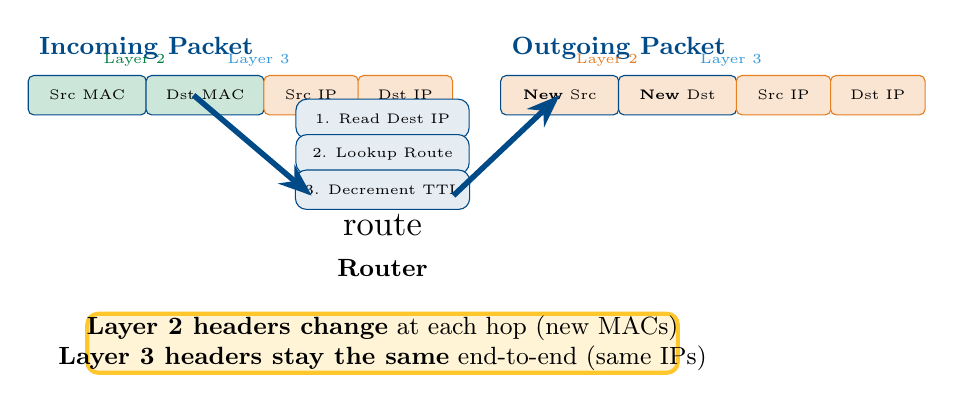
\begin{tikzpicture}[scale=0.75]
            % Left side - incoming packet
            \node[font=\small\bfseries, rctcblue] at (-4,3) {Incoming Packet};
            
            % Frame structure - incoming
            \node[pktseg, minimum width=1.5cm, fill=networkgreen!20] (srcmac1) at (-5,2.2) {\tiny Src MAC};
            \node[pktseg, minimum width=1.5cm, fill=networkgreen!20, right=-0.5pt of srcmac1] (dstmac1) {\tiny Dst MAC};
            \node[pktseg highlight, minimum width=1.2cm, right=-0.5pt of dstmac1] (srcip1) {\tiny Src IP};
            \node[pktseg highlight, minimum width=1.2cm, right=-0.5pt of srcip1] (dstip1) {\tiny Dst IP};
            
            % Router
            \node[router] (rtr) at (0,0) {\iconrouter[1cm]};
            \node[font=\small\bfseries, below=0.1cm of rtr] {Router};
            
            % Process steps inside router area
            \node[draw=rctcblue, fill=rctcblue!10, rounded corners, font=\tiny, align=center,
                  minimum width=2.2cm, minimum height=0.5cm] at (0,1.8) {1. Read Dest IP};
            \node[draw=rctcblue, fill=rctcblue!10, rounded corners, font=\tiny, align=center,
                  minimum width=2.2cm, minimum height=0.5cm] at (0,1.2) {2. Lookup Route};
            \node[draw=rctcblue, fill=rctcblue!10, rounded corners, font=\tiny, align=center,
                  minimum width=2.2cm, minimum height=0.5cm] at (0,0.6) {3. Decrement TTL};
            
            % Right side - outgoing packet
            \node[font=\small\bfseries, rctcblue] at (4,3) {Outgoing Packet};
            
            % Frame structure - outgoing (new MACs, same IPs)
            \node[pktseg, minimum width=1.5cm, fill=aborange!20] (srcmac2) at (3,2.2) {\tiny \textbf{New} Src};
            \node[pktseg, minimum width=1.5cm, fill=aborange!20, right=-0.5pt of srcmac2] (dstmac2) {\tiny \textbf{New} Dst};
            \node[pktseg highlight, minimum width=1.2cm, right=-0.5pt of dstmac2] (srcip2) {\tiny Src IP};
            \node[pktseg highlight, minimum width=1.2cm, right=-0.5pt of srcip2] (dstip2) {\tiny Dst IP};
            
            % Arrows
            \draw[-{Stealth}, line width=2pt, rctcblue] (-3.2,2.2) -- (-1.2,0.5);
            \draw[-{Stealth}, line width=2pt, rctcblue] (1.2,0.5) -- (3,2.2);
            
            % Key insight box at bottom
            \draw[fill=rctcgold!20, draw=rctcgold, line width=1.5pt, rounded corners]
                (-5,-1.5) rectangle (5,-2.5);
            \node[font=\small, align=center] at (0,-2) {
                \textbf{Layer 2 headers change} at each hop (new MACs) \\
                \textbf{Layer 3 headers stay the same} end-to-end (same IPs)
            };
            
            % Labels for MAC areas
            \node[font=\tiny, networkgreen] at (-4.2,2.8) {Layer 2};
            \node[font=\tiny, ipblue] at (-2.1,2.8) {Layer 3};
            \node[font=\tiny, aborange] at (3.8,2.8) {Layer 2};
            \node[font=\tiny, ipblue] at (5.9,2.8) {Layer 3};
        \end{tikzpicture}
    \end{center}
\end{frame}

% =============================================================================
% SLIDE 10: Fragmentation and MTU
% =============================================================================
\begin{frame}{Fragmentation and MTU}
    \begin{columns}[T]
        \begin{column}{0.48\textwidth}
            \begin{itemize}
                \item \keyterm{MTU} (Maximum Transmission Unit) is the largest packet size a link can carry.
                \item Standard Ethernet MTU: \textbf{1500 bytes}.
                \item If packet $>$ MTU, router must \keyterm{fragment} it into smaller pieces.
                \item Fragments are reassembled at the \textbf{destination}.
            \end{itemize}
            
            \vspace{0.3em}
            \begin{alertblock}{Problems with Fragmentation}
                \small
                \begin{itemize}\setlength{\itemsep}{1pt}
                    \item Adds processing overhead
                    \item If one fragment lost, entire packet must be retransmitted
                    \item Slower overall performance
                \end{itemize}
            \end{alertblock}
        \end{column}
        \begin{column}{0.48\textwidth}
            \begin{center}
                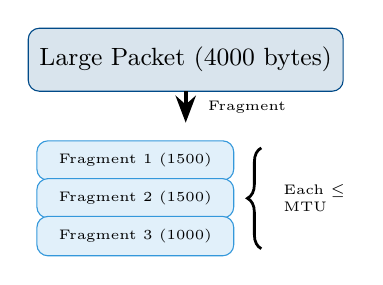
\begin{tikzpicture}[scale=0.8]
                    % Large packet
                    \node[draw=rctcblue, fill=rctcblue!15, minimum width=4cm, minimum height=0.8cm,
                          rounded corners, font=\small] (big) at (0,2.5) {Large Packet (4000 bytes)};
                    
                    % Arrow down
                    \draw[-{Stealth}, line width=1.5pt] (0,2) -- (0,1.5);
                    \node[font=\tiny, right] at (0.2,1.75) {Fragment};
                    
                    % Fragments
                    \node[draw=ipblue, fill=ipblue!15, minimum width=2.5cm, minimum height=0.5cm,
                          rounded corners, font=\tiny] (f1) at (-0.8,0.9) {Fragment 1 (1500)};
                    \node[draw=ipblue, fill=ipblue!15, minimum width=2.5cm, minimum height=0.5cm,
                          rounded corners, font=\tiny] (f2) at (-0.8,0.3) {Fragment 2 (1500)};
                    \node[draw=ipblue, fill=ipblue!15, minimum width=2.5cm, minimum height=0.5cm,
                          rounded corners, font=\tiny] (f3) at (-0.8,-0.3) {Fragment 3 (1000)};
                    
                    % MTU label
                    \draw[decorate, decoration={brace, amplitude=5pt, mirror}, line width=1pt]
                        (1.2,1.1) -- (1.2,-0.5);
                    \node[font=\tiny, right, align=left] at (1.4,0.3) {Each $\leq$\\MTU};
                \end{tikzpicture}
            \end{center}
            
\articleonly{
\par\small\emph{This MTU fragmentation diagram shows the process when a packet (4000 bytes) exceeds the maximum transmission unit: the router splits it into three fragments, each fitting within the 1500-byte MTU limit (Fragment 1: 1500 bytes, Fragment 2: 1500 bytes, Fragment 3: 1000 bytes). A brace on the right indicates that each fragment must be at most MTU size. This splitting adds processing overhead; modern systems use Path MTU Discovery to find the smallest MTU along the entire path, avoiding fragmentation altogether.}\par
}
            
            \vspace{0.2em}
            \begin{exampleblock}{Path MTU Discovery}
                \small
                Modern systems discover the smallest MTU along the entire path to avoid fragmentation.
            \end{exampleblock}
        \end{column}
    \end{columns}
\end{frame}

% =============================================================================
% SLIDE 11: Case Study - Westley's Journey to Florin
% =============================================================================
\begin{frame}{Case Study: Westley's Journey to Florin}
    \begin{casestudy}{Westley's Journey to Florin}
        \small
        Westley is sending a message from the Pirate Ship network (\texttt{172.16.0.0/24}) to Princess Buttercup at Castle Florin (\texttt{10.0.0.0/24}). The ship's router has this routing table:
        
        \vspace{0.2em}
        \footnotesize
        \begin{center}
            \begin{tabular}{l l l}
                \toprule
                \textbf{Network} & \textbf{Next Hop} & \textbf{Type} \\
                \midrule
                172.16.0.0/24 & Directly Connected & Direct \\
                10.0.0.0/24 & 192.168.50.1 & Static \\
                0.0.0.0/0 & 203.0.113.1 & Default \\
                \bottomrule
            \end{tabular}
        \end{center}
        
        \small
        Westley's PC: \texttt{172.16.0.25} \quad Buttercup's PC: \texttt{10.0.0.100}
    \end{casestudy}
    
    \begin{block}{Review Questions}
        \small
        \begin{enumerate}\setlength{\itemsep}{1pt}
            \item Which routing table entry will the router use for Westley's packet?
            \item What is the next hop IP address?
            \item What would happen if someone deleted the \texttt{10.0.0.0/24} entry?
        \end{enumerate}
    \end{block}
\end{frame}

% =============================================================================
% SLIDE 12: Case Study Solution - Westley's Journey to Florin
% =============================================================================
\begin{frame}{Case Study Solution: Westley's Journey to Florin}
    \begin{casesolution}{Westley's Journey to Florin}
        \small
        \begin{enumerate}\setlength{\itemsep}{1pt}
            \item Router uses \textbf{10.0.0.0/24}---longest prefix match for \texttt{10.0.0.100}.
            \item Next hop is \textbf{192.168.50.1} (path to Castle Florin).
            \item If deleted, router uses \textbf{default route} (\texttt{0.0.0.0/0}) via \texttt{203.0.113.1}---a longer path through the kingdom!
        \end{enumerate}
    \end{casesolution}
    
    \begin{center}
        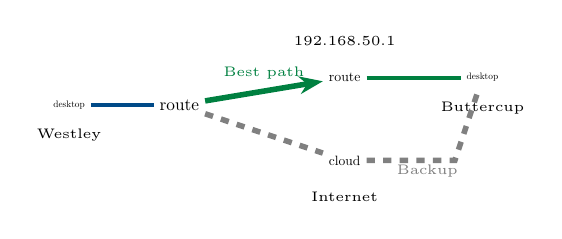
\begin{tikzpicture}[scale=0.7]
            % Pirate Ship
            \node[pc] (westley) at (0,0) {\iconpc[0.4cm]};
            \node[font=\tiny, below=0.05cm of westley] {Westley};
            
            \node[router] (shiprtr) at (2,0) {\iconrouter[0.5cm]};
            
            % Direct path
            \node[router] (rtr2) at (5,0.5) {\iconrouter[0.4cm]};
            \node[font=\tiny, above] at (5,0.9) {192.168.50.1};
            
            \node[pc] (buttercup) at (7.5,0.5) {\iconpc[0.4cm]};
            \node[font=\tiny, below=0.05cm of buttercup] {Buttercup};
            
            % Default path (longer)
            \node[cloud] (cloud) at (5,-1) {\iconcloud[0.4cm]};
            \node[font=\tiny, below] at (5,-1.4) {Internet};
            
            % Connections
            \draw[ethernet noarrow] (westley) -- (shiprtr);
            \draw[ethernet, networkgreen, line width=2pt] (shiprtr) -- (rtr2) node[midway, above, font=\tiny] {Best path};
            \draw[ethernet noarrow, networkgreen] (rtr2) -- (buttercup);
            
            \draw[wan noarrow, dashed, gray] (shiprtr) -- (cloud);
            \draw[wan noarrow, dashed, gray] (cloud) -- (7,-1) -- (buttercup);
            \node[font=\tiny, gray] at (6.5,-1.2) {Backup};
        \end{tikzpicture}
    \end{center}
    
    \begin{alertblock}{Key Lesson}
        \small
        ``As you wish!'' Specific routes always win over the default. Without proper entries, packets may take the long way---or never arrive!
    \end{alertblock}
\end{frame}

% =============================================================================
% SLIDE 13: Basic Router Configuration
% =============================================================================
\section{Router Configuration and Tools}
\subsection{Static Routing and Diagnostics}

\articleonly{
This section focuses on practical router setup, route verification, and path diagnostics using common operational tools.
}

\begin{frame}{Basic Router Configuration}
    \begin{columns}[T]
        \begin{column}{0.48\textwidth}
            \begin{block}{Essential Settings}
                \small
                \begin{itemize}\setlength{\itemsep}{2pt}
                    \item \textbf{Hostname} -- Identify the router
                    \item \textbf{Interface IPs} -- Address each port
                    \item \textbf{Enable interfaces} -- \texttt{no shutdown}
                    \item \textbf{Routes} -- Static and/or default
                    \item \textbf{Passwords} -- Secure access
                \end{itemize}
            \end{block}
            
            \vspace{0.2em}
            \begin{alertblock}{Two Configuration Methods}
                \small
                \textbf{CLI}: Command-line interface (Cisco IOS) \\
                \textbf{GUI}: Web-based management interface
            \end{alertblock}
        \end{column}
        \begin{column}{0.48\textwidth}
            \begin{block}{Sample CLI Commands}
                \ttfamily\scriptsize
                Router> enable \\
                Router\# configure terminal \\
                Router(config)\# hostname Florin-GW \\
                Florin-GW(config)\# interface g0/0 \\
                Florin-GW(config-if)\# ip address \\ 
                \quad 192.168.1.1 255.255.255.0 \\
                Florin-GW(config-if)\# no shutdown \\
                Florin-GW(config-if)\# exit \\
                Florin-GW(config)\# ip route 0.0.0.0 \\
                \quad 0.0.0.0 203.0.113.1
            \end{block}
            
            \vspace{0.2em}
            \begin{exampleblock}{Tip}
                \small
                Always save config: \texttt{copy run start}
            \end{exampleblock}
        \end{column}
    \end{columns}
\end{frame}

% =============================================================================
% SLIDE 14: Routing Table Tools
% =============================================================================
\begin{frame}{Routing Table Tools}
    \begin{columns}[T]
        \begin{column}{0.48\textwidth}
            \begin{block}{Cisco IOS Commands}
                \small
                \texttt{\textbf{show ip route}} \\
                Display full routing table
                
                \vspace{0.2em}
                \texttt{\textbf{show ip route} \textit{network}} \\
                Show specific route entry
                
                \vspace{0.2em}
                \texttt{\textbf{show ip interface brief}} \\
                Interface status summary
                
                \vspace{0.2em}
                \texttt{\textbf{show running-config}} \\
                View current configuration
            \end{block}
        \end{column}
        \begin{column}{0.48\textwidth}
            \begin{block}{Windows / Linux Commands}
                \small
                \texttt{\textbf{route print}} (Windows) \\
                \texttt{\textbf{netstat -r}} (Windows/Linux) \\
                Display host routing table
                
                \vspace{0.2em}
                \texttt{\textbf{ip route}} (Linux) \\
                Modern Linux routing display
                
                \vspace{0.2em}
                \texttt{\textbf{netstat -rn}} \\
                Numeric output (no DNS lookup)
            \end{block}
            
            \vspace{0.2em}
            \begin{exampleblock}{Quick Check}
                \small
                Use \texttt{ip route get \textit{IP}} on Linux to see which route would be used for a specific destination.
            \end{exampleblock}
        \end{column}
    \end{columns}
\end{frame}

% =============================================================================
% SLIDE 15: tracert and traceroute
% =============================================================================
\begin{frame}{tracert and traceroute}
    \begin{columns}[T]
        \begin{column}{0.42\textwidth}
            \begin{itemize}
                \item Shows the \textbf{path} packets take to a destination.
                \item Uses \keyterm{TTL manipulation}:
                    \begin{itemize}
                        \scriptsize
                        \item Send packet with TTL=1
                        \item First router sends back error
                        \item Increment TTL, repeat
                    \end{itemize}
                \item Each router returns \textbf{ICMP Time Exceeded}.
                \item \texttt{tracert} (Windows) \\
                      \texttt{traceroute} (Linux/Mac)
            \end{itemize}
            
            \vspace{0.2em}
            \begin{alertblock}{Use Cases}
                \small
                Find where packets get stuck, identify slow links, verify routing path.
            \end{alertblock}
        \end{column}
        \begin{column}{0.55\textwidth}
            \begin{center}
                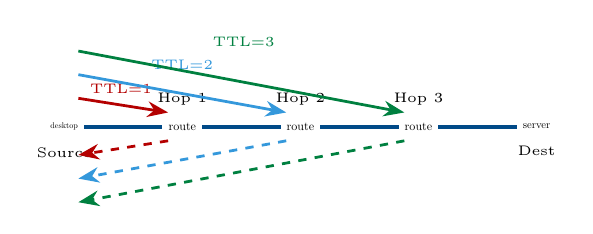
\begin{tikzpicture}[scale=0.6]
                    % Source
                    \node[pc] (src) at (0,0) {\iconpc[0.35cm]};
                    \node[font=\tiny, below=0.02cm of src] {Source};
                    
                    % Routers
                    \node[router] (r1) at (2.5,0) {\iconrouter[0.35cm]};
                    \node[font=\tiny, above=0.02cm of r1] {Hop 1};
                    
                    \node[router] (r2) at (5,0) {\iconrouter[0.35cm]};
                    \node[font=\tiny, above=0.02cm of r2] {Hop 2};
                    
                    \node[router] (r3) at (7.5,0) {\iconrouter[0.35cm]};
                    \node[font=\tiny, above=0.02cm of r3] {Hop 3};
                    
                    % Destination
                    \node[server] (dst) at (10,0) {\iconserver[0.35cm]};
                    \node[font=\tiny, below=0.02cm of dst] {Dest};
                    
                    % Connections
                    \draw[ethernet noarrow] (src) -- (r1) -- (r2) -- (r3) -- (dst);
                    
                    % TTL arrows (simplified)
                    \draw[-{Stealth}, alertred, line width=1pt] (0.3,0.6) -- (2.2,0.3);
                    \node[font=\tiny, alertred] at (1.2,0.8) {TTL=1};
                    \draw[-{Stealth}, alertred, dashed, line width=1pt] (2.2,-0.3) -- (0.3,-0.6);
                    
                    \draw[-{Stealth}, ipblue, line width=1pt] (0.3,1.1) -- (4.7,0.3);
                    \node[font=\tiny, ipblue] at (2.5,1.3) {TTL=2};
                    \draw[-{Stealth}, ipblue, dashed, line width=1pt] (4.7,-0.3) -- (0.3,-1.1);
                    
                    \draw[-{Stealth}, networkgreen, line width=1pt] (0.3,1.6) -- (7.2,0.3);
                    \node[font=\tiny, networkgreen] at (3.8,1.8) {TTL=3};
                    \draw[-{Stealth}, networkgreen, dashed, line width=1pt] (7.2,-0.3) -- (0.3,-1.6);
                \end{tikzpicture}
            \end{center}
            
\articleonly{
\par\small\emph{This traceroute diagram shows TTL-based path discovery: a source PC sends probes with incrementing TTL values (colored arrows labeled TTL=1, 2, 3) toward destination server through three intermediate routers. Each router decrements TTL; when TTL reaches zero, the router responds with its address and timing. Dashed return arrows show ICMP responses from each hop revealing the complete path with latency measurements, helping diagnose routing problems.}\par
}
            
            \vspace{0.3em}
            \begin{block}{Sample Output}
                \ttfamily\small
                \begin{tabular}{r l l l l}
                    1 & 2ms & 1ms & 1ms & 192.168.1.1 \\
                    2 & 10ms & 9ms & 11ms & 10.0.0.1 \\
                    3 & 15ms & 14ms & 15ms & 203.0.113.50 \\
                \end{tabular}
            \end{block}
        \end{column}
    \end{columns}
\end{frame}

% =============================================================================
% SLIDE 16: Dynamic Routing Protocols Overview
% =============================================================================
\section{Dynamic Routing Protocols}
\subsection{RIP, EIGRP, OSPF, and BGP}

\articleonly{
Dynamic routing protocols exchange topology information automatically and select best paths based on protocol metrics and policies.
}

\begin{frame}{Dynamic Routing Protocols Overview}
    \begin{columns}[T]
        \begin{column}{0.48\textwidth}
            \begin{block}{Why Dynamic Routing?}
                \small
                \begin{itemize}\setlength{\itemsep}{2pt}
                    \item Static routes don't adapt to failures
                    \item Large networks have hundreds of routes
                    \item Dynamic protocols \textbf{share route info automatically}
                    \item Network changes propagate without admin intervention
                \end{itemize}
            \end{block}
            
            \vspace{0.2em}
            \begin{alertblock}{Two Categories}
                \small
                \textbf{IGP} (Interior Gateway Protocol) \\
                Within an organization: RIP, OSPF, EIGRP
                
                \vspace{0.2em}
                \textbf{EGP} (Exterior Gateway Protocol) \\
                Between organizations: BGP
            \end{alertblock}
        \end{column}
        \begin{column}{0.48\textwidth}
            \begin{center}
                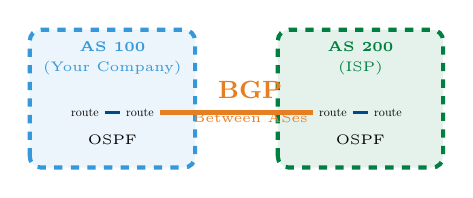
\begin{tikzpicture}[scale=0.7]
                    % AS 1
                    \draw[dashed, ipblue, line width=1.5pt, rounded corners, fill=ipblue!10] 
                        (-0.5,-0.5) rectangle (2.5,2);
                    \node[font=\tiny\bfseries, ipblue] at (1,1.7) {AS 100};
                    \node[font=\tiny, ipblue] at (1,1.3) {(Your Company)};
                    
                    \node[router] (r1) at (0.5,0.5) {\iconrouter[0.35cm]};
                    \node[router] (r2) at (1.5,0.5) {\iconrouter[0.35cm]};
                    \draw[ethernet noarrow, line width=1pt] (r1) -- (r2);
                    \node[font=\tiny] at (1,0) {OSPF};
                    
                    % AS 2
                    \draw[dashed, networkgreen, line width=1.5pt, rounded corners, fill=networkgreen!10] 
                        (4,-0.5) rectangle (7,2);
                    \node[font=\tiny\bfseries, networkgreen] at (5.5,1.7) {AS 200};
                    \node[font=\tiny, networkgreen] at (5.5,1.3) {(ISP)};
                    
                    \node[router] (r3) at (5,0.5) {\iconrouter[0.35cm]};
                    \node[router] (r4) at (6,0.5) {\iconrouter[0.35cm]};
                    \draw[ethernet noarrow, line width=1pt] (r3) -- (r4);
                    \node[font=\tiny] at (5.5,0) {OSPF};
                    
                    % BGP connection
                    \draw[wan noarrow, aborange, line width=2pt] (r2) -- (r3);
                    \node[font=\small\bfseries, aborange] at (3.5,0.9) {BGP};
                    \node[font=\tiny, aborange] at (3.5,0.4) {Between ASes};
                \end{tikzpicture}
            \end{center}
            
\articleonly{
\par\small\emph{This diagram shows two autonomous systems (ASes) separated by administrative boundaries: AS 100 (Your Company, blue) runs OSPF internally with two routers exchanging routes efficiently. AS 200 (ISP, green) also runs OSPF internally. The critical orange WAN link between them carries BGP (Border Gateway Protocol), the inter-AS protocol that allows organizations to exchange routing information at the internet's administrative borders. OSPF handles fast convergence and optimal paths within an organization, while BGP provides intentional, policy-based routing between organizations.}\par
}
            
            \vspace{0.3em}
            \begin{exampleblock}{Autonomous System (AS)}
                \small
                A network under single administrative control. Each AS has a unique number (ASN).
            \end{exampleblock}
        \end{column}
    \end{columns}
\end{frame}

% =============================================================================
% SLIDE 17: RIP and EIGRP
% =============================================================================
\begin{frame}{RIP and EIGRP}
    \begin{columns}[T]
        \begin{column}{0.48\textwidth}
            \begin{block}{RIP (Routing Information Protocol)}
                \small
                \begin{itemize}\setlength{\itemsep}{2pt}
                    \item Simple, easy to configure
                    \item Uses \textbf{hop count} as metric
                    \item Maximum 15 hops (16 = unreachable)
                    \item Broadcasts updates every 30 seconds
                    \item Slow convergence
                \end{itemize}
                
                \vspace{0.2em}
                \textbf{Best for}: Small, simple networks
            \end{block}
            
            \vspace{0.2em}
            \begin{alertblock}{RIP Limitation}
                \small
                Hop count ignores link speed! A 10 Gbps path with 3 hops loses to a 1 Mbps path with 2 hops.
            \end{alertblock}
        \end{column}
        \begin{column}{0.48\textwidth}
            \begin{block}{EIGRP (Enhanced Interior Gateway RP)}
                \small
                \begin{itemize}\setlength{\itemsep}{2pt}
                    \item Cisco-developed (now partially open)
                    \item Uses \textbf{bandwidth + delay} for metric
                    \item Fast convergence
                    \item Only sends updates when changes occur
                    \item Supports unequal-cost load balancing
                \end{itemize}
                
                \vspace{0.2em}
                \textbf{Best for}: Cisco enterprise networks
            \end{block}
            
            \vspace{0.2em}
            \begin{exampleblock}{EIGRP Advantage}
                \small
                Keeps backup routes ready---failover is nearly instant!
            \end{exampleblock}
        \end{column}
    \end{columns}
\end{frame}

% =============================================================================
% SLIDE 18: OSPF (Open Shortest Path First)
% =============================================================================
\begin{frame}{OSPF (Open Shortest Path First)}
    \begin{columns}[T]
        \begin{column}{0.48\textwidth}
            \begin{itemize}
                \item \textbf{Industry standard} (open protocol)
                \item Uses \keyterm{cost} based on bandwidth
                \item Creates complete network map (\keyterm{link-state})
                \item Fast convergence
                \item Supports \textbf{hierarchical design} with areas
            \end{itemize}
            
            \vspace{0.2em}
            \begin{block}{OSPF Cost Formula}
                \centering
                Cost = $\dfrac{10^8}{\text{bandwidth (bps)}}$
                
                \vspace{0.3em}
                \small
                \begin{tabular}{l r}
                    100 Mbps & Cost = 1 \\
                    10 Mbps & Cost = 10 \\
                    1 Gbps & Cost = 1 \\
                \end{tabular}
            \end{block}
        \end{column}
        \begin{column}{0.48\textwidth}
            \begin{center}
                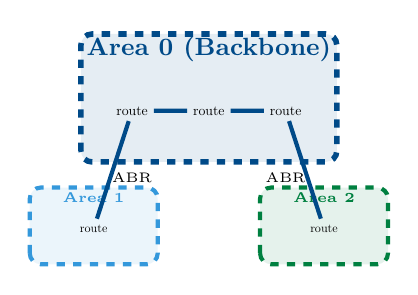
\begin{tikzpicture}[scale=0.65]
                    % Area 0 (backbone)
                    \draw[dashed, rctcblue, line width=2pt, rounded corners, fill=rctcblue!10] 
                        (0.5,0) rectangle (5.5,2.5);
                    \node[font=\small\bfseries, rctcblue] at (3,2.2) {Area 0 (Backbone)};
                    
                    \node[router] (r1) at (1.5,1) {\iconrouter[0.4cm]};
                    \node[router] (r2) at (3,1) {\iconrouter[0.4cm]};
                    \node[router] (r3) at (4.5,1) {\iconrouter[0.4cm]};
                    \draw[ethernet noarrow] (r1) -- (r2) -- (r3);
                    
                    % Area 1
                    \draw[dashed, ipblue, line width=1.5pt, rounded corners, fill=ipblue!10] 
                        (-0.5,-2) rectangle (2,-0.5);
                    \node[font=\tiny\bfseries, ipblue] at (0.75,-0.7) {Area 1};
                    \node[router] (r4) at (0.75,-1.3) {\iconrouter[0.35cm]};
                    \draw[ethernet noarrow] (r1) -- (r4);
                    \node[font=\tiny] at (1.5,-0.3) {ABR};
                    
                    % Area 2
                    \draw[dashed, networkgreen, line width=1.5pt, rounded corners, fill=networkgreen!10] 
                        (4,-2) rectangle (6.5,-0.5);
                    \node[font=\tiny\bfseries, networkgreen] at (5.25,-0.7) {Area 2};
                    \node[router] (r5) at (5.25,-1.3) {\iconrouter[0.35cm]};
                    \draw[ethernet noarrow] (r3) -- (r5);
                    \node[font=\tiny] at (4.5,-0.3) {ABR};
                \end{tikzpicture}
            \end{center}

\articleonly{
\par\small\emph{This diagram illustrates the relationship between routing protocols and administrative autonomy: Company network (AS 100, blue) runs OSPF internally with two connected routers communicating via OSPF, while ISP network (AS 200, green) also uses OSPF internally with its routers. The critical orange WAN link between them runs BGP (Border Gateway Protocol), which is the inter-AS protocol that exchanges routes between autonomous systems at the administrative boundary. This architecture shows how OSPF handles intra-AS routing efficiency while BGP manages inter-AS reachability across the internet.}\par
}
            
            \vspace{0.2em}
            \begin{exampleblock}{ABR}
                \small
                \textbf{Area Border Router} connects areas to the backbone (Area 0).
            \end{exampleblock}
        \end{column}
    \end{columns}
\end{frame}

% =============================================================================
% SLIDE 19: BGP (Border Gateway Protocol)
% =============================================================================
\begin{frame}{BGP (Border Gateway Protocol)}
    \begin{columns}[T]
        \begin{column}{0.48\textwidth}
            \begin{itemize}
                \item The \textbf{routing protocol of the Internet}
                \item Connects different organizations (ASes)
                \item \keyterm{Path vector} protocol
                \item Uses \textbf{policies} more than metrics
                \item Very slow, deliberate convergence
            \end{itemize}
            
            \vspace{0.2em}
            \begin{block}{When to Use BGP}
                \small
                \begin{itemize}\setlength{\itemsep}{1pt}
                    \item Connecting to multiple ISPs
                    \item Running your own AS
                    \item Need fine control over routing policy
                \end{itemize}
            \end{block}
            
            \vspace{0.2em}
            \begin{alertblock}{Warning}
                \small
                BGP misconfigurations can break parts of the Internet! Handle with care.
            \end{alertblock}
        \end{column}
        \begin{column}{0.48\textwidth}
            \begin{center}
                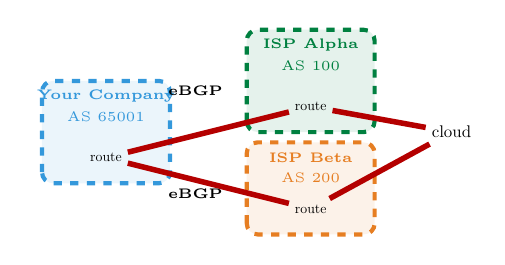
\begin{tikzpicture}[scale=0.65]
                    % Your company
                    \draw[dashed, ipblue, line width=1.5pt, rounded corners, fill=ipblue!10] 
                        (0,1) rectangle (2.5,3);
                    \node[font=\tiny\bfseries, ipblue] at (1.25,2.7) {Your Company};
                    \node[font=\tiny, ipblue] at (1.25,2.3) {AS 65001};
                    \node[router] (r1) at (1.25,1.5) {\iconrouter[0.4cm]};
                    
                    % ISP 1
                    \draw[dashed, networkgreen, line width=1.5pt, rounded corners, fill=networkgreen!10] 
                        (4,2) rectangle (6.5,4);
                    \node[font=\tiny\bfseries, networkgreen] at (5.25,3.7) {ISP Alpha};
                    \node[font=\tiny, networkgreen] at (5.25,3.3) {AS 100};
                    \node[router] (r2) at (5.25,2.5) {\iconrouter[0.4cm]};
                    
                    % ISP 2
                    \draw[dashed, aborange, line width=1.5pt, rounded corners, fill=aborange!10] 
                        (4,0) rectangle (6.5,1.8);
                    \node[font=\tiny\bfseries, aborange] at (5.25,1.5) {ISP Beta};
                    \node[font=\tiny, aborange] at (5.25,1.1) {AS 200};
                    \node[router] (r3) at (5.25,0.5) {\iconrouter[0.4cm]};
                    
                    % BGP connections
                    \draw[wan noarrow, line width=2pt] (r1) -- (r2);
                    \draw[wan noarrow, line width=2pt] (r1) -- (r3);
                    
                    \node[font=\tiny\bfseries] at (3,2.8) {eBGP};
                    \node[font=\tiny\bfseries] at (3,0.8) {eBGP};
                    
                    % Internet cloud
                    \node[cloud] (cloud) at (8,2) {\iconcloud[0.5cm]};
                    \draw[wan noarrow] (r2) -- (cloud);
                    \draw[wan noarrow] (r3) -- (cloud);
                \end{tikzpicture}
            \end{center}
            
\articleonly{
\par\small\emph{This multihoming diagram demonstrates redundancy through dual ISP connections: a company router connects to both ISP Alpha (AS 100, green) and ISP Beta (AS 200, orange) via separate eBGP connections, allowing traffic to the internet cloud to split between them. Both ISPs connect to the internet, providing path redundancy and load distribution. If one ISP link fails, traffic automatically reroutes through the other, ensuring business continuity. This architecture is typical of enterprises requiring high availability.}\par
}
            
            \vspace{0.2em}
            \begin{exampleblock}{Multihoming}
                \small
                Connecting to multiple ISPs provides redundancy and load balancing.
            \end{exampleblock}
        \end{column}
    \end{columns}
\end{frame}

% =============================================================================
% SLIDE 20: Route Selection and Administrative Distance
% =============================================================================
\begin{frame}{Route Selection and Administrative Distance}
    \begin{columns}[T]
        \begin{column}{0.48\textwidth}
            \begin{block}{Routing Protocol Metrics}
                \small
                \begin{tabular}{l l}
                    \toprule
                    \textbf{Protocol} & \textbf{Metric} \\
                    \midrule
                    RIP & Hop count \\
                    EIGRP & Bandwidth + delay \\
                    OSPF & Cost (bandwidth) \\
                    BGP & Path attributes \\
                    \bottomrule
                \end{tabular}
            \end{block}
            
            \vspace{0.3em}
            \begin{alertblock}{What If Multiple Protocols?}
                \small
                When the same route is learned from different protocols, \textbf{Administrative Distance} decides which to trust.
            \end{alertblock}
        \end{column}
        \begin{column}{0.48\textwidth}
            \begin{block}{Administrative Distance (AD)}
                \small
                Lower AD = more trusted
                
                \vspace{0.2em}
                \begin{tabular}{l r}
                    \toprule
                    \textbf{Route Source} & \textbf{AD} \\
                    \midrule
                    Directly Connected & 0 \\
                    Static Route & 1 \\
                    EIGRP (internal) & 90 \\
                    OSPF & 110 \\
                    RIP & 120 \\
                    External EIGRP & 170 \\
                    Unknown & 255 \\
                    \bottomrule
                \end{tabular}
            \end{block}
            
            \vspace{0.2em}
            \begin{exampleblock}{Example}
                \small
                If OSPF (AD 110) and RIP (AD 120) both know a route, OSPF wins!
            \end{exampleblock}
        \end{column}
    \end{columns}
\end{frame}

% =============================================================================
% SLIDE 21: Case Study - Inigo's Path to Count Rugen
% =============================================================================
\begin{frame}{Case Study: Inigo's Path to Count Rugen}
    \begin{casestudy}{Inigo's Path to Count Rugen}
        \small
        Inigo Montoya has configured routers to help him find Count Rugen (the six-fingered man). His router has learned two paths to Rugen's network (\texttt{10.20.30.0/24}):
        
        \vspace{0.3em}
        \footnotesize
        \begin{center}
            \begin{tabular}{l l l l}
                \toprule
                \textbf{Protocol} & \textbf{Next Hop} & \textbf{Metric} & \textbf{AD} \\
                \midrule
                OSPF & 192.168.1.1 & Cost: 20 & 110 \\
                RIP & 192.168.2.1 & Hops: 3 & 120 \\
                \bottomrule
            \end{tabular}
        \end{center}
        
        \vspace{0.2em}
        \small
        Both paths are currently working. Inigo needs to reach Rugen as quickly as possible!
    \end{casestudy}
    
    \begin{block}{Review Questions}
        \small
        \begin{enumerate}\setlength{\itemsep}{1pt}
            \item Which route will the router prefer and why?
            \item What is Administrative Distance and how does it apply here?
            \item If the OSPF path fails, what happens?
        \end{enumerate}
    \end{block}
\end{frame}

% =============================================================================
% SLIDE 22: Case Study Solution - Inigo's Path to Count Rugen
% =============================================================================
\begin{frame}{Case Study Solution: Inigo's Path to Count Rugen}
    \begin{casesolution}{Inigo's Path to Count Rugen}
        \small
        \begin{enumerate}\setlength{\itemsep}{1pt}
            \item Router prefers \textbf{OSPF route}---AD of 110 beats RIP's AD of 120.
            \item \textbf{Administrative Distance} is a ``trustworthiness'' rating. Lower AD = more trusted. When multiple protocols know a route, lowest AD wins.
            \item If OSPF fails, router automatically uses \textbf{RIP route} as backup!
        \end{enumerate}
    \end{casesolution}
    
    \begin{center}
        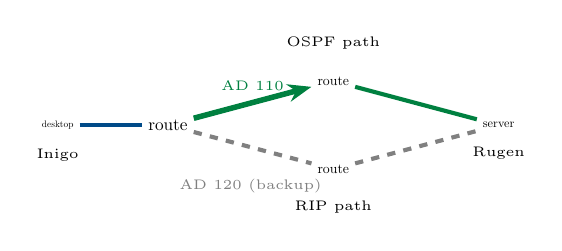
\begin{tikzpicture}[scale=0.7]
            % Inigo
            \node[pc] (inigo) at (0,0) {\iconpc[0.4cm]};
            \node[font=\tiny, below=0.05cm of inigo] {Inigo};
            
            \node[router] (rtr1) at (2,0) {\iconrouter[0.5cm]};
            
            % OSPF path (preferred)
            \node[router] (rtr2) at (5,0.8) {\iconrouter[0.4cm]};
            \node[font=\tiny, above] at (5,1.2) {OSPF path};
            
            % RIP path (backup)
            \node[router] (rtr3) at (5,-0.8) {\iconrouter[0.4cm]};
            \node[font=\tiny, below] at (5,-1.2) {RIP path};
            
            % Count Rugen
            \node[server] (rugen) at (8,0) {\iconserver[0.4cm]};
            \node[font=\tiny, below=0.05cm of rugen] {Rugen};
            
            % Connections
            \draw[ethernet noarrow] (inigo) -- (rtr1);
            \draw[ethernet, networkgreen, line width=2pt] (rtr1) -- (rtr2) node[midway, above, font=\tiny] {AD 110};
            \draw[ethernet noarrow, networkgreen] (rtr2) -- (rugen);
            
            \draw[ethernet noarrow, dashed, gray] (rtr1) -- (rtr3);
            \draw[ethernet noarrow, dashed, gray] (rtr3) -- (rugen);
            \node[font=\tiny, gray] at (3.5,-1.1) {AD 120 (backup)};
        \end{tikzpicture}
    \end{center}
    
    \begin{alertblock}{Key Lesson}
        \small
        ``Hello. My name is Inigo Montoya...'' Administrative Distance determines which protocol to trust. The backup route is ready if the primary fails!
    \end{alertblock}
\end{frame}

% =============================================================================
% SLIDE 23: Edge Routers and Network Boundaries
% =============================================================================
\section{Edge Services and Translation}
\subsection{NAT, PAT, and Firewalls}

\articleonly{
At the network edge, address translation and filtering enforce policy while enabling internal hosts to reach external networks.
}

\begin{frame}{Edge Routers and Network Boundaries}
    \begin{columns}[T]
        \begin{column}{0.48\textwidth}
            \begin{itemize}
                \item \keyterm{Edge router} connects internal network to outside (ISP).
                \item Also called: border router, gateway router.
                \item Key responsibilities:
                    \begin{itemize}
                        \small
                        \item Route between internal and external
                        \item Apply \textbf{NAT} (translate IPs)
                        \item First line of security (ACLs)
                        \item Connect to ISP via WAN link
                    \end{itemize}
            \end{itemize}
            
            \vspace{0.2em}
            \begin{alertblock}{Demarcation Point}
                \small
                The boundary where your network ends and the ISP's begins. Usually at the edge router.
            \end{alertblock}
        \end{column}
        \begin{column}{0.48\textwidth}
            \begin{center}
                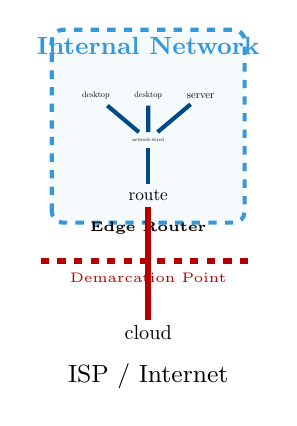
\begin{tikzpicture}[scale=0.7]
                    % Internal network
                    \draw[dashed, ipblue, line width=1.5pt, rounded corners, fill=ipblue!5] 
                        (-0.5,-1.5) rectangle (3,2);
                    \node[font=\small\bfseries, ipblue] at (1.25,1.7) {Internal Network};
                    
                    \node[pc] (pc1) at (0.3,0.8) {\iconpc[0.35cm]};
                    \node[pc] (pc2) at (1.25,0.8) {\iconpc[0.35cm]};
                    \node[server] (srv) at (2.2,0.8) {\iconserver[0.35cm]};
                    
                    \node[switch] (sw) at (1.25,0) {\iconswitch[0.4cm]};
                    \draw[ethernet noarrow] (pc1) -- (sw);
                    \draw[ethernet noarrow] (pc2) -- (sw);
                    \draw[ethernet noarrow] (srv) -- (sw);
                    
                    % Edge router
                    \node[router] (edge) at (1.25,-1) {\iconrouter[0.5cm]};
                    \node[font=\tiny\bfseries] at (1.25,-1.6) {Edge Router};
                    \draw[ethernet noarrow] (sw) -- (edge);
                    
                    % Demarcation line
                    \draw[line width=2pt, alertred, dashed] (-0.7,-2.2) -- (3.2,-2.2);
                    \node[font=\tiny, alertred] at (1.25,-2.5) {Demarcation Point};
                    
                    % ISP Cloud
                    \node[cloud] (cloud) at (1.25,-3.5) {\iconcloud[0.6cm]};
                    \node[font=\small, below=0.1cm of cloud] {ISP / Internet};
                    \draw[wan noarrow, line width=2pt] (edge) -- (cloud);
                \end{tikzpicture}
            \end{center}
        \end{column}
    \end{columns}
\end{frame}

% =============================================================================
% SLIDE 24: Network Address Translation (NAT)
% =============================================================================
\begin{frame}{Network Address Translation (NAT)}
    \begin{columns}[T]
        \begin{column}{0.48\textwidth}
            \begin{itemize}
                \item \keyterm{NAT} translates private IPs to public IPs.
                \item Allows many internal devices to share limited public addresses.
                \item Essential because IPv4 addresses are exhausted!
                \item Performed by edge router or firewall.
            \end{itemize}
            
            \vspace{0.2em}
            \begin{block}{NAT Terminology}
                \small
                \begin{itemize}\setlength{\itemsep}{1pt}
                    \item \textbf{Inside Local}: Private IP (192.168.1.10)
                    \item \textbf{Inside Global}: Public IP seen by internet
                    \item \textbf{Outside}: External destination
                \end{itemize}
            \end{block}
        \end{column}
        \begin{column}{0.48\textwidth}
            \begin{center}
                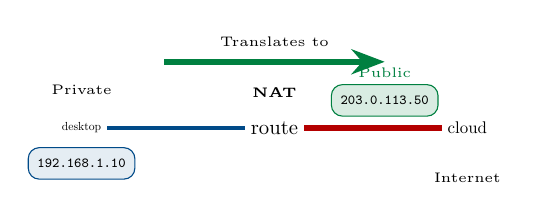
\begin{tikzpicture}[scale=0.7]
                    % Internal
                    \node[pc] (pc) at (0,0) {\iconpc[0.5cm]};
                    \node[ipbox, font=\tiny\ttfamily, below=0.1cm of pc] {192.168.1.10};
                    \node[font=\tiny] at (0,0.7) {Private};
                    
                    % NAT Router
                    \node[router] (nat) at (3.5,0) {\iconrouter[0.6cm]};
                    \node[font=\tiny\bfseries, above=0.1cm of nat] {NAT};
                    
                    % External
                    \node[cloud] (cloud) at (7,0) {\iconcloud[0.5cm]};
                    \node[font=\tiny, below=0.3cm of cloud] {Internet};
                    
                    % Connections
                    \draw[ethernet noarrow] (pc) -- (nat);
                    \draw[wan noarrow] (nat) -- (cloud);
                    
                    % Translation arrow
                    \draw[-{Stealth}, line width=2pt, networkgreen] (1.5,1.2) -- (5.5,1.2);
                    \node[font=\tiny, above] at (3.5,1.3) {Translates to};
                    
                    % Public IP shown
                    \node[ipbox, font=\tiny\ttfamily, fill=networkgreen!15, draw=networkgreen] 
                        at (5.5,0.5) {203.0.113.50};
                    \node[font=\tiny, networkgreen] at (5.5,1) {Public};
                \end{tikzpicture}
            \end{center}
            
\articleonly{
\par\small\emph{This NAT translation diagram illustrates the core concept: a PC on private network (192.168.1.10 on left, blue) connects through a NAT router to the internet. The green arrow labeled "Translates to" shows that the router dynamically rewrites the source address in outgoing packets, changing the private address to a public address (203.0.113.50, green) that the ISP assigned. Return traffic is automatically reverse-translated back to the private address. This allows multiple private devices to share a single public IP address, saving address space and providing network privacy.}\par
}
            
            \vspace{0.3em}
            \begin{exampleblock}{Why NAT Matters}
                \small
                Your home network might have 20 devices, but your ISP only gives you \textbf{one} public IP. NAT makes this work!
            \end{exampleblock}
        \end{column}
    \end{columns}
\end{frame}

% =============================================================================
% SLIDE 25: NAT Types
% =============================================================================
\begin{frame}{NAT Types}
    \begin{columns}[T]
        \begin{column}{0.48\textwidth}
            \begin{block}{Static NAT}
                \small
                \begin{itemize}\setlength{\itemsep}{2pt}
                    \item One private IP $\leftrightarrow$ One public IP
                    \item Permanent, fixed mapping
                    \item Use: Servers needing consistent public address
                \end{itemize}
                
                \vspace{0.2em}
                \centering
                \texttt{192.168.1.10 $\leftrightarrow$ 203.0.113.10}
            \end{block}
            
            \vspace{0.2em}
            \begin{block}{Dynamic NAT}
                \small
                \begin{itemize}\setlength{\itemsep}{2pt}
                    \item Pool of private $\rightarrow$ Pool of public
                    \item First-come, first-served
                    \item Mapping changes over time
                    \item Use: When you have several public IPs
                \end{itemize}
            \end{block}
        \end{column}
        \begin{column}{0.48\textwidth}
            \begin{center}
                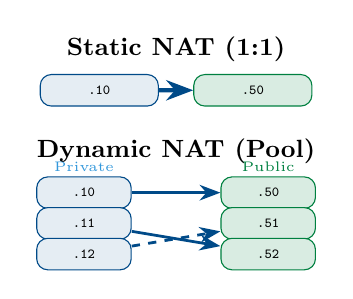
\begin{tikzpicture}[scale=0.65]
                    % Static NAT
                    \node[font=\small\bfseries] at (0,3) {Static NAT (1:1)};
                    \node[ipbox, font=\tiny\ttfamily, minimum width=1.5cm] (s1) at (-1.5,2.2) {.10};
                    \node[ipbox, font=\tiny\ttfamily, minimum width=1.5cm, fill=networkgreen!15, draw=networkgreen] (s2) at (1.5,2.2) {.50};
                    \draw[-{Stealth}, line width=1.5pt, rctcblue] (s1) -- (s2);
                    
                    % Dynamic NAT
                    \node[font=\small\bfseries] at (0,1) {Dynamic NAT (Pool)};
                    \node[ipbox, font=\tiny\ttfamily, minimum width=1.2cm] (d1) at (-1.8,0.2) {.10};
                    \node[ipbox, font=\tiny\ttfamily, minimum width=1.2cm] (d2) at (-1.8,-0.4) {.11};
                    \node[ipbox, font=\tiny\ttfamily, minimum width=1.2cm] (d3) at (-1.8,-1) {.12};
                    
                    \node[ipbox, font=\tiny\ttfamily, minimum width=1.2cm, fill=networkgreen!15, draw=networkgreen] (p1) at (1.8,0.2) {.50};
                    \node[ipbox, font=\tiny\ttfamily, minimum width=1.2cm, fill=networkgreen!15, draw=networkgreen] (p2) at (1.8,-0.4) {.51};
                    \node[ipbox, font=\tiny\ttfamily, minimum width=1.2cm, fill=networkgreen!15, draw=networkgreen] (p3) at (1.8,-1) {.52};
                    
                    \draw[-{Stealth}, line width=1pt, rctcblue] (d1) -- (p1);
                    \draw[-{Stealth}, line width=1pt, rctcblue] (d2) -- (p3);
                    \draw[-{Stealth}, line width=1pt, rctcblue, dashed] (d3) -- (p2);
                    
                    % Labels
                    \node[font=\tiny, ipblue] at (-1.8,0.7) {Private};
                    \node[font=\tiny, networkgreen] at (1.8,0.7) {Public};
                \end{tikzpicture}
            \end{center}
            
\articleonly{
\par\small\emph{This NAT types diagram compares two translation approaches: Static NAT (top, 1:1 mapping) translates one private IP (.10) to exactly one public IP (.50) with a fixed, permanent relationship—good for servers requiring consistent addresses. Dynamic NAT (bottom, pool) maps multiple private IPs (.10, .11, .12) to a pool of public IPs (.50, .51, .52) using temporary associations—when a device connects, it gets assigned the next available public IP, and when disconnected, that public IP returns to the pool. Both require sufficient public IPs; neither scales to thousands of devices on a single public address.}\par
}
            
            \vspace{0.2em}
            \begin{alertblock}{Limitation}
                \small
                Both Static and Dynamic NAT require one public IP per active connection. Not scalable!
            \end{alertblock}
        \end{column}
    \end{columns}
\end{frame}

% =============================================================================
% SLIDE 26: PAT (Port Address Translation)
% =============================================================================
\begin{frame}{PAT: Port Address Translation}
    \begin{columns}[T]
        \begin{column}{0.45\textwidth}
            \begin{itemize}
                \item \keyterm{PAT} = Many private IPs share ONE public IP
                \item Uses \textbf{port numbers} to track connections
                \item Also called: NAT Overload, NAPT
                \item \textbf{Most common} type in homes and businesses
            \end{itemize}
            
            \vspace{0.2em}
            \begin{block}{How PAT Works}
                \small
                \begin{enumerate}\setlength{\itemsep}{1pt}
                    \item Host sends packet (src port 12345)
                    \item Router changes src IP to public
                    \item Router assigns unique port (e.g., 40001)
                    \item Tracks mapping in NAT table
                    \item Return traffic uses port to find host
                \end{enumerate}
            \end{block}
        \end{column}
        \begin{column}{0.52\textwidth}
            \begin{center}
                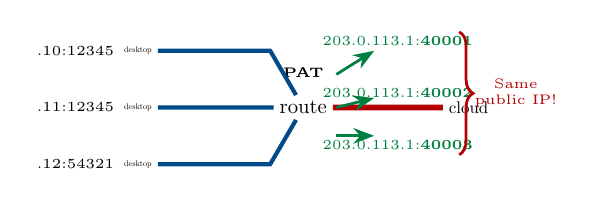
\begin{tikzpicture}[scale=0.6]
                    % Internal hosts
                    \node[pc] (pc1) at (0,2) {\iconpc[0.35cm]};
                    \node[font=\tiny, left] at (-0.3,2) {.10:12345};
                    
                    \node[pc] (pc2) at (0,0.8) {\iconpc[0.35cm]};
                    \node[font=\tiny, left] at (-0.3,0.8) {.11:12345};
                    
                    \node[pc] (pc3) at (0,-0.4) {\iconpc[0.35cm]};
                    \node[font=\tiny, left] at (-0.3,-0.4) {.12:54321};
                    
                    % PAT Router
                    \node[router] (pat) at (3.5,0.8) {\iconrouter[0.6cm]};
                    \node[font=\tiny\bfseries, above=0.1cm of pat] {PAT};
                    
                    % Internet
                    \node[cloud] (cloud) at (7,0.8) {\iconcloud[0.5cm]};
                    
                    % Connections
                    \draw[ethernet noarrow] (pc1) -- (2.8,2) -- (pat);
                    \draw[ethernet noarrow] (pc2) -- (pat);
                    \draw[ethernet noarrow] (pc3) -- (2.8,-0.4) -- (pat);
                    \draw[wan noarrow] (pat) -- (cloud);
                    
                    % Translated addresses
                    \node[font=\tiny, networkgreen, align=left] at (5.5,2.2) {203.0.113.1:\textbf{40001}};
                    \node[font=\tiny, networkgreen, align=left] at (5.5,1.1) {203.0.113.1:\textbf{40002}};
                    \node[font=\tiny, networkgreen, align=left] at (5.5,0) {203.0.113.1:\textbf{40003}};
                    
                    \draw[-{Stealth}, line width=1pt, networkgreen] (4.2,1.5) -- (5,2);
                    \draw[-{Stealth}, line width=1pt, networkgreen] (4.2,0.8) -- (5,1);
                    \draw[-{Stealth}, line width=1pt, networkgreen] (4.2,0.2) -- (5,0.2);
                    
                    % One public IP label
                    \draw[decorate, decoration={brace, amplitude=5pt}, line width=1pt, alertred]
                        (6.8,2.4) -- (6.8,-0.2);
                    \node[font=\tiny, alertred, align=center] at (8,1.1) {Same\\public IP!};
                \end{tikzpicture}
            \end{center}
            
\articleonly{
\par\small\emph{This Port Address Translation (PAT) diagram illustrates how multiple private devices share a single public IP: three PCs (192.168.1.10:50001, 192.168.1.11:40002, 192.168.1.12:54321) all pass through a PAT router and emerge as port multiplexed connections under the same public IP (203.0.113.1) but with different port numbers (:40001, :40002, :40003). The red brace on the right emphasizes that all three distinct internal connections appear to the internet as one IP address with different ports. This is why home networks with ~65,000 available ports can support thousands of simultaneous connections with just one public IP address.}\par
}
            
            \vspace{0.2em}
            \begin{exampleblock}{Capacity}
                \small
                With ~65,000 available ports, one public IP can support thousands of simultaneous connections!
            \end{exampleblock}
        \end{column}
    \end{columns}
\end{frame}

% =============================================================================
% SLIDE 27: Firewall Uses and Types
% =============================================================================
\begin{frame}{Firewall Uses and Types}
    \begin{columns}[T]
        \begin{column}{0.48\textwidth}
            \begin{block}{What Firewalls Do}
                \small
                \begin{itemize}\setlength{\itemsep}{2pt}
                    \item Filter traffic based on rules
                    \item Block unauthorized access
                    \item Allow legitimate traffic through
                    \item Log security events
                    \item Enforce security policies
                \end{itemize}
            \end{block}
            
            \vspace{0.2em}
            \begin{alertblock}{Default Behavior}
                \small
                Most firewalls: \textbf{Deny all, permit by exception}. Only explicitly allowed traffic passes.
            \end{alertblock}
        \end{column}
        \begin{column}{0.48\textwidth}
            \begin{block}{Firewall Types}
                \small
                \begin{itemize}\setlength{\itemsep}{3pt}
                    \item \textbf{Packet Filtering} \\
                        {\scriptsize Checks IP/port only (stateless)}
                    \item \textbf{Stateful Inspection} \\
                        {\scriptsize Tracks connection state}
                    \item \textbf{Application Layer} \\
                        {\scriptsize Inspects content (Layer 7)}
                    \item \textbf{Next-Gen (NGFW)} \\
                        {\scriptsize All above + IPS, deep inspection}
                \end{itemize}
            \end{block}
            
            \vspace{0.2em}
            \begin{exampleblock}{Trend}
                \small
                Modern networks use NGFW for comprehensive protection.
            \end{exampleblock}
        \end{column}
    \end{columns}
\end{frame}

% =============================================================================
% SLIDE 28: Firewall Placement and DMZ
% =============================================================================
\begin{frame}{Firewall Placement and DMZ}
    \begin{columns}[T]
        \begin{column}{0.42\textwidth}
            \begin{block}{Placement Options}
                \small
                \begin{itemize}\setlength{\itemsep}{2pt}
                    \item \textbf{Perimeter}: Between LAN and internet
                    \item \textbf{Internal}: Between network segments
                    \item \textbf{Host-based}: On individual devices
                \end{itemize}
            \end{block}
            
            \vspace{0.2em}
            \begin{block}{DMZ (Demilitarized Zone)}
                \small
                \begin{itemize}\setlength{\itemsep}{2pt}
                    \item Screened subnet for public servers
                    \item Web, email, DNS servers go here
                    \item Isolated from internal LAN
                    \item If compromised, LAN still protected
                \end{itemize}
            \end{block}
        \end{column}
        \begin{column}{0.55\textwidth}
            \begin{center}
                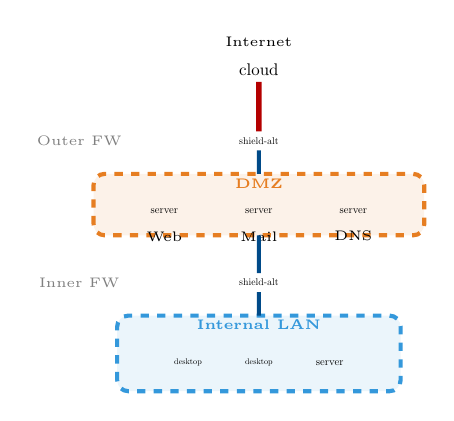
\begin{tikzpicture}[scale=0.6]
                    % Internet
                    \node[cloud] (inet) at (4,4) {\iconcloud[0.5cm]};
                    \node[font=\tiny] at (4,4.6) {Internet};
                    
                    % Outer Firewall
                    \node[firewall] (fw1) at (4,2.5) {\iconfirewall[0.5cm]};
                    \draw[wan noarrow] (inet) -- (fw1);
                    
                    % DMZ
                    \draw[dashed, aborange, line width=1.5pt, rounded corners, fill=aborange!10] 
                        (0.5,0.5) rectangle (7.5,1.8);
                    \node[font=\tiny\bfseries, aborange] at (4,1.6) {DMZ};
                    
                    \node[server] (web) at (2,1) {\iconserver[0.35cm]};
                    \node[font=\tiny, below=0.02cm of web] {Web};
                    
                    \node[server] (mail) at (4,1) {\iconserver[0.35cm]};
                    \node[font=\tiny, below=0.02cm of mail] {Mail};
                    
                    \node[server] (dns) at (6,1) {\iconserver[0.35cm]};
                    \node[font=\tiny, below=0.02cm of dns] {DNS};
                    
                    \draw[ethernet noarrow] (fw1) -- (4,1.8);
                    
                    % Inner Firewall
                    \node[firewall] (fw2) at (4,-0.5) {\iconfirewall[0.5cm]};
                    \draw[ethernet noarrow] (4,0.5) -- (fw2);
                    
                    % Internal LAN
                    \draw[dashed, ipblue, line width=1.5pt, rounded corners, fill=ipblue!10] 
                        (1,-2.8) rectangle (7,-1.2);
                    \node[font=\tiny\bfseries, ipblue] at (4,-1.4) {Internal LAN};
                    
                    \node[pc] (pc1) at (2.5,-2.2) {\iconpc[0.35cm]};
                    \node[pc] (pc2) at (4,-2.2) {\iconpc[0.35cm]};
                    \node[server] (srv) at (5.5,-2.2) {\iconserver[0.35cm]};
                    
                    \draw[ethernet noarrow] (fw2) -- (4,-1.2);
                    
                    % Labels
                    \node[font=\tiny, gray] at (0.2,2.5) {Outer FW};
                    \node[font=\tiny, gray] at (0.2,-0.5) {Inner FW};
                \end{tikzpicture}
            \end{center}
            
            \begin{alertblock}{Defense in Depth}
                \small
                Multiple firewall layers provide better protection than a single firewall.
            \end{alertblock}
        \end{column}
    \end{columns}
\end{frame}

% =============================================================================
% SLIDE 29: Introduction to VLANs
% =============================================================================
\section{VLAN Segmentation and Trunking}
\subsection{VLAN Design and Security}

\articleonly{
This section introduces VLAN segmentation, trunking, and security practices for multi-segment switched environments.
}

\begin{frame}{Introduction to VLANs}
    \begin{columns}[T]
        \begin{column}{0.48\textwidth}
            \begin{itemize}
                \item \keyterm{VLAN} = Virtual Local Area Network
                \item Logically separates one physical switch into multiple \textbf{broadcast domains}.
                \item Devices on different VLANs cannot communicate directly---need a router.
                \item Configured per switch port.
            \end{itemize}
            
            \vspace{0.2em}
            \begin{block}{Benefits of VLANs}
                \small
                \begin{itemize}\setlength{\itemsep}{1pt}
                    \item \textbf{Security}: Isolate sensitive traffic
                    \item \textbf{Performance}: Reduce broadcast traffic
                    \item \textbf{Flexibility}: Group by function, not location
                    \item \textbf{Cost}: One switch, many networks
                \end{itemize}
            \end{block}
        \end{column}
        \begin{column}{0.48\textwidth}
            \begin{center}
                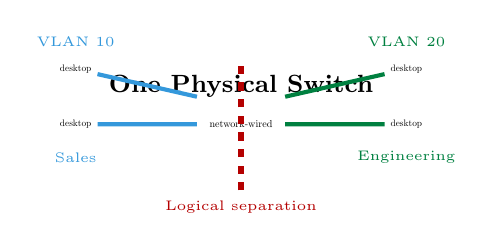
\begin{tikzpicture}[scale=0.7]
                    % Switch
                    \node[switch] (sw) at (3,1.5) {\iconswitch[0.8cm]};
                    \node[font=\small\bfseries, above=0.1cm of sw] {One Physical Switch};
                    
                    % VLAN 10 (Sales)
                    \node[pc] (pc1) at (0,2.5) {\iconpc[0.4cm]};
                    \node[pc] (pc2) at (0,1.5) {\iconpc[0.4cm]};
                    \draw[ethernet noarrow, ipblue, line width=1.5pt] (pc1) -- (2.2,2);
                    \draw[ethernet noarrow, ipblue, line width=1.5pt] (pc2) -- (2.2,1.5);
                    \node[font=\tiny, ipblue] at (0,3) {VLAN 10};
                    \node[font=\tiny, ipblue] at (0,0.9) {Sales};
                    
                    % VLAN 20 (Engineering)
                    \node[pc] (pc3) at (6,2.5) {\iconpc[0.4cm]};
                    \node[pc] (pc4) at (6,1.5) {\iconpc[0.4cm]};
                    \draw[ethernet noarrow, networkgreen, line width=1.5pt] (pc3) -- (3.8,2);
                    \draw[ethernet noarrow, networkgreen, line width=1.5pt] (pc4) -- (3.8,1.5);
                    \node[font=\tiny, networkgreen] at (6,3) {VLAN 20};
                    \node[font=\tiny, networkgreen] at (6,0.9) {Engineering};
                    
                    % Separation indicator
                    \draw[dashed, alertred, line width=2pt] (3,0.3) -- (3,2.7);
                    \node[font=\tiny, alertred] at (3,0) {Logical separation};
                \end{tikzpicture}
            \end{center}
            
\articleonly{
\par\small\emph{This VLAN isolation diagram shows a single physical switch (center) containing two logically separate networks: VLAN 10 Sales (blue, left with two PCs) and VLAN 20 Engineering (green, right with two PCs). Despite being on the same physical switch hardware, a red dashed line represents the logical separation—devices in VLAN 10 cannot communicate directly with VLAN 20 devices. This Layer 2 isolation provides network segmentation for security and traffic management, though cross-VLAN communication requires a Layer 3 router.}\par
}
            
            \vspace{0.2em}
            \begin{alertblock}{Key Point}
                \small
                VLANs create Layer 2 isolation. Cross-VLAN traffic requires Layer 3 routing!
            \end{alertblock}
        \end{column}
    \end{columns}
\end{frame}

% =============================================================================
% SLIDE 30: VLAN Trunking and 802.1Q
% =============================================================================
\begin{frame}{VLAN Trunking and 802.1Q}
    \begin{columns}[T]
        \begin{column}{0.48\textwidth}
            \begin{block}{The Problem}
                \small
                How do VLANs span multiple switches? We need a way to carry VLAN info between switches.
            \end{block}
            
            \vspace{0.2em}
            \begin{block}{Trunk Ports}
                \small
                \begin{itemize}\setlength{\itemsep}{2pt}
                    \item Carry traffic for \textbf{multiple VLANs}
                    \item Connect switches to switches
                    \item Connect switches to routers
                    \item Use \keyterm{802.1Q tagging}
                \end{itemize}
            \end{block}
            
            \vspace{0.2em}
            \begin{alertblock}{Access vs Trunk}
                \small
                \textbf{Access port}: One VLAN, untagged \\
                \textbf{Trunk port}: Multiple VLANs, tagged
            \end{alertblock}
        \end{column}
        \begin{column}{0.48\textwidth}
            \begin{center}
                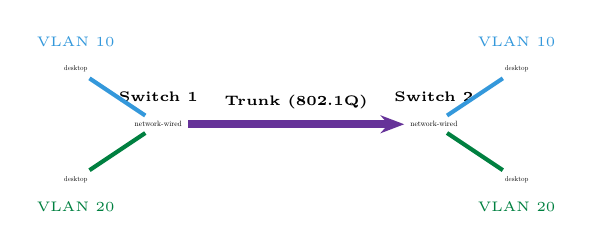
\begin{tikzpicture}[scale=0.7]
                    % Switch 1
                    \node[switch] (sw1) at (0,1.5) {\iconswitch[0.6cm]};
                    \node[font=\tiny\bfseries, above=0.05cm of sw1] {Switch 1};
                    
                    % Switch 2
                    \node[switch] (sw2) at (5,1.5) {\iconswitch[0.6cm]};
                    \node[font=\tiny\bfseries, above=0.05cm of sw2] {Switch 2};
                    
                    % Trunk link
                    \draw[trunk, line width=3pt] (sw1) -- (sw2);
                    \node[font=\tiny\bfseries] at (2.5,1.9) {Trunk (802.1Q)};
                    
                    % VLAN 10 hosts
                    \node[pc] (pc1) at (-1.5,2.5) {\iconpc[0.3cm]};
                    \node[pc] (pc2) at (6.5,2.5) {\iconpc[0.3cm]};
                    \draw[ethernet noarrow, ipblue] (pc1) -- (sw1);
                    \draw[ethernet noarrow, ipblue] (sw2) -- (pc2);
                    \node[font=\tiny, ipblue] at (-1.5,3) {VLAN 10};
                    \node[font=\tiny, ipblue] at (6.5,3) {VLAN 10};
                    
                    % VLAN 20 hosts
                    \node[pc] (pc3) at (-1.5,0.5) {\iconpc[0.3cm]};
                    \node[pc] (pc4) at (6.5,0.5) {\iconpc[0.3cm]};
                    \draw[ethernet noarrow, networkgreen] (pc3) -- (sw1);
                    \draw[ethernet noarrow, networkgreen] (sw2) -- (pc4);
                    \node[font=\tiny, networkgreen] at (-1.5,0) {VLAN 20};
                    \node[font=\tiny, networkgreen] at (6.5,0) {VLAN 20};
                \end{tikzpicture}
            \end{center}
            
\articleonly{
\par\small\emph{This VLAN trunking diagram shows two physical switches (Switch 1 on left, Switch 2 on right) connected by a thick orange trunk link carrying both VLAN 10 (blue) and VLAN 20 (green) traffic simultaneously. Despite being on different physical switches, VLAN 10 devices on the left connect logically to VLAN 10 devices on the right, and VLAN 20 devices span both switches—maintaining logical separation across physical infrastructure. The 802.1Q protocol tags each frame with a 12-bit VLAN ID, allowing the trunk to multiplex multiple VLANs. This enables geographically distributed network segmentation where logically grouped devices remain isolated from other VLANs regardless of physical switch location.}\par
}
            
            \vspace{0.3em}
            \begin{block}{802.1Q Tag}
                \small
                Adds 4-byte tag to Ethernet frame:
                \begin{itemize}\setlength{\itemsep}{0pt}
                    \item \textbf{VLAN ID}: 12 bits (1--4094)
                    \item \textbf{Priority}: 3 bits (QoS)
                \end{itemize}
            \end{block}
        \end{column}
    \end{columns}
\end{frame}

% =============================================================================
% SLIDE 31: Voice VLANs
% =============================================================================
\begin{frame}{Voice VLANs}
    \begin{columns}[T]
        \begin{column}{0.48\textwidth}
            \begin{itemize}
                \item VoIP phones need \textbf{priority treatment} for quality calls.
                \item \keyterm{Voice VLAN} separates phone traffic from data traffic.
                \item One port supports both:
                    \begin{itemize}
                        \small
                        \item Data VLAN (for PC)
                        \item Voice VLAN (for phone)
                    \end{itemize}
                \item Phone traffic gets higher QoS priority.
            \end{itemize}
            
            \vspace{0.2em}
            \begin{block}{Configuration Example}
                \ttfamily\small
                switchport mode access \\
                switchport access vlan 10 \\
                switchport voice vlan 50
            \end{block}
        \end{column}
        \begin{column}{0.48\textwidth}
            \begin{center}
                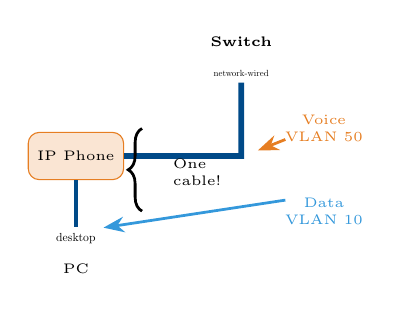
\begin{tikzpicture}[scale=0.7]
                    % Switch
                    \node[switch] (sw) at (3,2) {\iconswitch[0.7cm]};
                    \node[font=\tiny\bfseries, above=0.1cm of sw] {Switch};
                    
                    % IP Phone
                    \node[draw=aborange, fill=aborange!20, rounded corners, 
                          minimum width=1cm, minimum height=0.6cm, font=\tiny] 
                          (phone) at (0,0.5) {IP Phone};
                    
                    % PC connected to phone
                    \node[pc] (pc) at (0,-1) {\iconpc[0.5cm]};
                    \node[font=\tiny, below=0.05cm of pc] {PC};
                    
                    % Connections
                    \draw[ethernet noarrow, line width=2pt] (sw) -- (3,0.5) -- (phone);
                    \draw[ethernet noarrow] (phone) -- (pc);
                    
                    % VLAN labels
                    \node[font=\tiny, aborange, align=center] at (4.5,1) {Voice\\VLAN 50};
                    \node[font=\tiny, ipblue, align=center] at (4.5,-0.5) {Data\\VLAN 10};
                    
                    \draw[-{Stealth}, aborange, line width=1pt] (3.8,0.8) -- (3.3,0.6);
                    \draw[-{Stealth}, ipblue, line width=1pt] (3.8,-0.3) -- (0.5,-0.8);
                    
                    % Single cable note
                    \draw[decorate, decoration={brace, amplitude=5pt, mirror}, line width=1pt]
                        (1.2,1) -- (1.2,-0.5);
                    \node[font=\tiny, align=left] at (2.2,0.2) {One\\cable!};
                \end{tikzpicture}
            \end{center}
            
\articleonly{
\par\small\emph{This Voice VLAN diagram shows how a single cable can carry both voice and data traffic: an IP phone sits at the center with a switch connection above and a PC plugged into the phone below, using just one physical cable from switch to phone. The phone tags traffic as Voice VLAN 50 (orange) destined to the switch, while the PC's data uses Data VLAN 10 (blue). The switch separates these two VLANs logically, giving voice traffic higher QoS priority. This converged network approach saves cabling costs and enables quality voice calls even when data traffic becomes heavy, as voice is sensitive to delay and jitter.}\par
}
            
            \vspace{0.3em}
            \begin{exampleblock}{Why Separate?}
                \small
                Voice is sensitive to delay and jitter. Separating it ensures calls stay clear even when data traffic is heavy.
            \end{exampleblock}
        \end{column}
    \end{columns}
\end{frame}

% =============================================================================
% SLIDE 32: Native VLAN and Security
% =============================================================================
\begin{frame}{Native VLAN and Security}
    \begin{columns}[T]
        \begin{column}{0.48\textwidth}
            \begin{block}{What is Native VLAN?}
                \small
                \begin{itemize}\setlength{\itemsep}{2pt}
                    \item Traffic on trunk that has \textbf{no 802.1Q tag}
                    \item Default: VLAN 1
                    \item Used for backward compatibility
                    \item Both ends of trunk must match!
                \end{itemize}
            \end{block}
            
            \vspace{0.2em}
            \begin{alertblock}{Security Risk}
                \small
                Attackers can exploit native VLAN mismatches to hop between VLANs. This is called \textbf{VLAN hopping}. Best practices:
                \begin{itemize}
                    \scriptsize
                    \item Change native VLAN from default
                    \item Use unused VLAN for native
                    \item Ensure both trunk ends match
                \end{itemize}
            \end{alertblock}
        \end{column}
        \begin{column}{0.48\textwidth}
            \begin{center}
                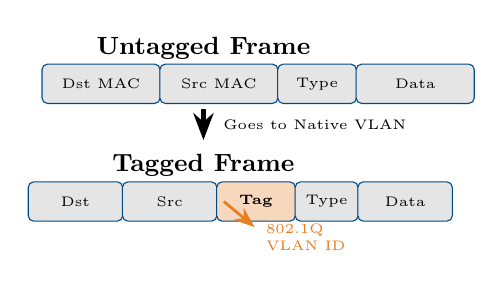
\begin{tikzpicture}[scale=0.65]
                    % Frame without tag
                    \node[font=\small\bfseries] at (2.5,3.5) {Untagged Frame};
                    \node[pktseg, minimum width=1.5cm, fill=gray!20] (dst) at (0.5,2.8) {\tiny Dst MAC};
                    \node[pktseg, minimum width=1.5cm, fill=gray!20, right=-0.5pt of dst] (src) {\tiny Src MAC};
                    \node[pktseg, minimum width=1cm, fill=gray!20, right=-0.5pt of src] (type) {\tiny Type};
                    \node[pktseg, minimum width=1.5cm, fill=gray!20, right=-0.5pt of type] (data) {\tiny Data};
                    
                    % Arrow
                    \draw[-{Stealth}, line width=1.5pt] (2.5,2.3) -- (2.5,1.7);
                    \node[font=\tiny, right] at (2.7,2) {Goes to Native VLAN};
                    
                    % Frame with tag
                    \node[font=\small\bfseries] at (2.5,1.2) {Tagged Frame};
                    \node[pktseg, minimum width=1.2cm, fill=gray!20] (dst2) at (0,0.5) {\tiny Dst};
                    \node[pktseg, minimum width=1.2cm, fill=gray!20, right=-0.5pt of dst2] (src2) {\tiny Src};
                    \node[pktseg, minimum width=1cm, fill=aborange!30, right=-0.5pt of src2] (tag) {\tiny \textbf{Tag}};
                    \node[pktseg, minimum width=0.8cm, fill=gray!20, right=-0.5pt of tag] (type2) {\tiny Type};
                    \node[pktseg, minimum width=1.2cm, fill=gray!20, right=-0.5pt of type2] (data2) {\tiny Data};
                    
                    % Tag detail
                    \draw[-{Stealth}, aborange, line width=1pt] (2.9,0.5) -- (3.5,0);
                    \node[font=\tiny, aborange, align=left] at (4.5,-0.2) {802.1Q\\VLAN ID};
                \end{tikzpicture}
            \end{center}
            
\articleonly{
\par\small\emph{This diagram contrasts untagged and tagged Ethernet frames: an untagged frame (top) carries only traditional Ethernet headers (Dst MAC, Src MAC, Type, Data) and is automatically assigned to the native VLAN when sent across a trunk. A tagged frame (bottom) inserts a 4-byte 802.1Q tag after the Src MAC field, containing the VLAN ID (12 bits) and Priority field (3 bits for QoS). Untagged frames bypass VLAN classification, while tagged frames are delivered to their specific VLAN. This mechanism allows switches to multiplex hundreds of VLANs across single trunk links by explicitly marking each frame with its VLAN membership.}\par
}
            
            \vspace{0.3em}
            \begin{exampleblock}{Configuration}
                \ttfamily\small
                switchport trunk native vlan 999
            \end{exampleblock}
            
            \vspace{0.2em}
            \begin{block}{VLAN 1 Concerns}
                \small
                VLAN 1 carries management traffic by default. Keep it separate from user data!
            \end{block}
        \end{column}
    \end{columns}
\end{frame}

% =============================================================================
% SLIDE 33: Case Study - Miracle Max's Potion Shop
% =============================================================================
\begin{frame}{Case Study: Miracle Max's Potion Shop}
    \begin{casestudy}{Miracle Max's Potion Shop}
        \small
        Miracle Max runs a potion shop with three departments, each on its own VLAN:
        
        \vspace{0.2em}
        \footnotesize
        \begin{center}
            \begin{tabular}{l l l}
                \toprule
                \textbf{Department} & \textbf{VLAN} & \textbf{Subnet} \\
                \midrule
                Potion Brewing & VLAN 10 & 192.168.10.0/24 \\
                Customer Sales & VLAN 20 & 192.168.20.0/24 \\
                Billing Office & VLAN 30 & 192.168.30.0/24 \\
                \bottomrule
            \end{tabular}
        \end{center}
        
        \vspace{0.2em}
        \small
        The Sales team (\texttt{192.168.20.50}) needs to check inventory on the Brewing server (\texttt{192.168.10.10}), but their packets aren't getting through!
    \end{casestudy}
    
    \begin{block}{Review Questions}
        \small
        \begin{enumerate}\setlength{\itemsep}{1pt}
            \item Why can't Sales communicate directly with Brewing?
            \item What device is needed to enable this communication?
            \item What is this process called?
        \end{enumerate}
    \end{block}
\end{frame}

% =============================================================================
% SLIDE 34: Case Study Solution - Miracle Max's Potion Shop
% =============================================================================
\begin{frame}[t,shrink=12]{Case Study Solution: Miracle Max's Potion Shop}
    \begin{casesolution}{Miracle Max's Potion Shop}
        \small
        \begin{enumerate}\setlength{\itemsep}{1pt}
            \item VLANs are separate broadcast domains---\textbf{Layer 2 isolation} prevents direct communication between VLANs.
            \item A \textbf{router} (or Layer 3 switch) is needed to route between VLANs.
            \item This is called \keyterm{inter-VLAN routing}.
        \end{enumerate}
    \end{casesolution}
    
    \begin{center}
        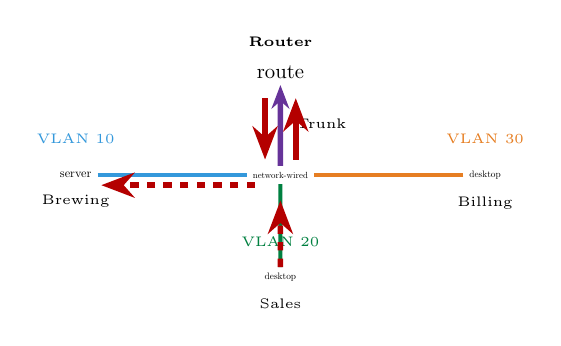
\begin{tikzpicture}[scale=0.65]
            % Switch
            \node[switch] (sw) at (4,0) {\iconswitch[0.7cm]};
            
            % Router
            \node[router] (rtr) at (4,2) {\iconrouter[0.6cm]};
            \node[font=\tiny\bfseries, above=0.05cm of rtr] {Router};
            \draw[trunk, line width=2pt] (sw) -- (rtr);
            \node[font=\tiny] at (4.8,1) {Trunk};
            
            % VLAN 10 - Brewing
            \node[server] (brew) at (0,0) {\iconserver[0.4cm]};
            \node[font=\tiny, below=0.02cm of brew] {Brewing};
            \node[font=\tiny, ipblue] at (0,0.7) {VLAN 10};
            \draw[ethernet noarrow, ipblue] (brew) -- (sw);
            
            % VLAN 20 - Sales
            \node[pc] (sales) at (4,-2) {\iconpc[0.4cm]};
            \node[font=\tiny, below=0.02cm of sales] {Sales};
            \node[font=\tiny, networkgreen] at (4,-1.3) {VLAN 20};
            \draw[ethernet noarrow, networkgreen] (sales) -- (sw);
            
            % VLAN 30 - Billing
            \node[pc] (bill) at (8,0) {\iconpc[0.4cm]};
            \node[font=\tiny, below=0.02cm of bill] {Billing};
            \node[font=\tiny, aborange] at (8,0.7) {VLAN 30};
            \draw[ethernet noarrow, aborange] (bill) -- (sw);
            
            % Traffic flow
            \draw[-{Stealth}, line width=2pt, alertred, dashed] (sales) -- (4,-0.5);
            \draw[-{Stealth}, line width=2pt, alertred] (4.3,0.3) -- (4.3,1.5);
            \draw[-{Stealth}, line width=2pt, alertred] (3.7,1.5) -- (3.7,0.3);
            \draw[-{Stealth}, line width=2pt, alertred, dashed] (3.5,-0.2) -- (0.5,-0.2);
        \end{tikzpicture}
    \end{center}
    
    \begin{alertblock}{Key Lesson}
        \small
        ``Have fun storming the castle!'' VLANs provide security through isolation, but inter-VLAN routing lets authorized traffic flow when needed.
    \end{alertblock}
\end{frame}

% =============================================================================
% SLIDE 35: Module 5.0 Summary
% =============================================================================
\section*{Module Summary}

\begin{frame}[t,allowframebreaks]{Module 5.0 Summary}
    \scriptsize
    \textbf{Key Concepts:}
    \begin{itemize}
        \item \keyterm{Routers} connect networks at Layer 3. \keyterm{Routing tables} store known destinations; \keyterm{longest prefix match} selects best route.
        \item \keyterm{Static routes}: Manually configured, predictable. \keyterm{Default route} (0.0.0.0/0) is gateway of last resort.
        \item Dynamic routing: \keyterm{RIP} (hop count, max 15), \keyterm{EIGRP} (Cisco, fast convergence), \keyterm{OSPF} (open standard, link-state), \keyterm{BGP} (internet backbone).
        \framebreak
        \item \keyterm{Administrative Distance (AD)} determines protocol trustworthiness: Direct (0) > Static (1) > EIGRP (90) > OSPF (110) > RIP (120).
        \item \keyterm{NAT} translates private IPs to public. Types: \keyterm{Static NAT} (1:1), \keyterm{Dynamic NAT} (pool), \keyterm{PAT} (many-to-one using ports).
        \item \keyterm{Firewalls} filter traffic: Packet filter, Stateful, Application-level, \keyterm{NGFW} (Next-Generation). \keyterm{DMZ} = screened subnet for servers.
    \end{itemize}
    \framebreak
    
    \vspace{0.3em}
    \textbf{VLANs \& Network Design:}
    \begin{itemize}
        \item \keyterm{VLANs} logically segment networks on one switch, creating separate broadcast domains for security, performance, and flexibility.
        \item \keyterm{802.1Q} tags frames with VLAN ID (1-4094). \keyterm{Trunk ports} carry multiple VLANs. \keyterm{Native VLAN}: untagged traffic.
        \item \keyterm{Voice VLANs} separate voice from data traffic, apply QoS priority (one port, two VLANs).
        \item \keyterm{Inter-VLAN routing} requires Layer 3 device (router or Layer 3 switch with \keyterm{SVI} - Switched Virtual Interface).
        \item \keyterm{Three-tier hierarchy}: \keyterm{Core} (backbone), \keyterm{Distribution} (policy/routing), \keyterm{Access} (end-device connection).
        \item \keyterm{Spine-leaf architecture}: Modern data center design with predictable latency and no oversubscription.
    \end{itemize}
\end{frame}

\articleonly{
\subsection*{Conclusion}
This module explored routing protocols, network address translation, firewalls, VLANs, and enterprise network design. You learned how routers make forwarding decisions, how dynamic routing protocols adapt to topology changes, how NAT/PAT conserve addresses, and how VLANs provide logical segmentation. In the next module, we'll examine network services including DHCP and DNS.
}

\end{document}
